\documentclass{wissdoc}
% Autor: Roland Bless 1996-2009, bless <at> kit.edu
% ----------------------------------------------------------------
% Diplomarbeit - Hauptdokument
% ----------------------------------------------------------------
%%
%% $Id: diplarb.tex 53 2009-12-10 12:23:37Z bless $
%%
% wissdoc Optionen: draft, relaxed, pdf --> siehe wissdoc.cls
% ------------------------------------------------------------------
% Weitere packages: (Dokumentation dazu durch "latex <package>.dtx")
\usepackage{bibgerm}
\usepackage[numbers,sort&compress]{natbib}
% \usepackage{varioref}
% \usepackage{verbatim}
% \usepackage{float}    %z.B. \floatstyle{ruled}\restylefloat{figure}
%\usepackage{subfigure}
\usepackage{subcaption}
\usepackage{listings}
% \usepackage{fancybox} % für schattierte,ovale Boxen etc.
% \usepackage{tabularx} % automatische Spaltenbreite
% \usepackage{supertab} % mehrseitige Tabellen
% \usepackage[svnon,svnfoot]{svnver} % SVN Versionsinformation 
%% ---------------- end of usepackages -------------

%\svnversion{$Id: diplarb.tex 53 2009-12-10 12:23:37Z bless $} % In case that you want to include version information in the footer

%% Informationen für die PDF-Datei
\hypersetup{
 pdfauthor={N.N.},
 pdftitle={Not set}
 pdfsubject={Not set},
 pdfkeywords={Not set}
}

% Macros, nicht unbedingt notwendig
%%%%%%%%%%%%%%%%%%%%%%%%%%%%%%%%%%%%%%%%%%%%%%%%%%%%%%%%%%
% macros.tex -- einige mehr oder weniger nuetzliche Makros
% Autor: Roland Bless 1998
%%%%%%%%%%%%%%%%%%%%%%%%%%%%%%%%%%%%%%%%%%%%%%%%%%%%%%%%%%
% $Id: macros.tex 33 2007-01-23 09:00:59Z bless $
%%%%%%%%%%%%%%%%%%%%%%%%%%%%%%%%%%%%%%%%%%%%%%%%%%%%%%%%%%


%%%%%%%%%%%%%%%%%%%%%%%
% Kommentare 
%%%%%%%%%%%%%%%%%%%%%%%
\ifnotdraftelse{
\newcommand{\Kommentar}[1]{}
}{\newcommand{\Kommentar}[1]{{\em #1}}}
% Alles innerhalb von \Hide{} oder \ignore{} 
% wird von LaTeX komplett ignoriert (wie ein Kommentar)
\newcommand{\Hide}[1]{}
\let\ignore\Hide

%%%%%%%%%%%%%%%%%%%%%%%%%
% Leere Seite ohne Seitennummer, wird aber gezaehlt
%%%%%%%%%%%%%%%%%%%%%%%%%

\newcommand{\leereseite}{% Leerseite ohne Seitennummer, nächste Seite rechts (wenn 2-seitig)
 \clearpage{\pagestyle{empty}\cleardoublepage}
}
%%%%%%%%%%%%%%%%%%%%%%%%%%
% Flattersatz rechts und Silbentrennung, Leerraum nach rechts maximal 1cm
%%%%%%%%%%%%%%%%%%%%%%%%%%
\makeatletter
\newcommand{\myraggedright}{%
 \let\\\@centercr\@rightskip 0pt plus 1cm
 \rightskip\@rightskip
  \leftskip\z@skip
  \parindent\z@
  \spaceskip=.3333em
  \xspaceskip=.5em}
\makeatother

\makeatletter
\newcommand{\mynewline}{%
 \@centercr\@rightskip 0pt plus 1cm
}
\makeatother


%%%%%%%%%%%%%%%%%%%%%%%%%%
% Für Index
%%%%%%%%%%%%%%%%%%%%%%%%%%
\makeatletter
\def\mydotfill{\leavevmode\xleaders\hb@xt@ .44em{\hss.\hss}\hfill\kern\z@}
\makeatother
\def\bold#1{{\bfseries #1}}
\newbox\dbox \setbox\dbox=\hbox to .4em{\hss.\hss} % dot box for leaders
\newskip\rrskipb \rrskipb=.5em plus3em % ragged right space before break
\newskip\rrskipa \rrskipa=-.17em plus -3em minus.11em % ditto, after
\newskip\rlskipa \rlskipa=0pt plus3em % ragged left space after break
\newskip\rlskipb \rlskipb=.33em plus-3em minus.11em % ragged left before break
\newskip\lskip \lskip=3.3\wd\dbox plus1fil minus.3\wd\dbox % for leaders
\newskip \lskipa \lskipa=-2.67em plus -3em minus.11em %after leaders
\mathchardef\rlpen=1000 \mathchardef\leadpen=600
\def\rrspace{\nobreak\hskip\rrskipb\penalty0\hskip\rrskipa}
\def\rlspace{\penalty\rlpen\hskip\rlskipb\vadjust{}\nobreak\hskip\rlskipa}
\let\indexbreak\rlspace
\def\raggedurl{\penalty10000 \hskip.5em plus15em \penalty0 \hskip-.17em plus-15em minus.11em}
\def\raggeditems{\nobreak\hskip\rrskipb \penalty\leadpen \hskip\rrskipa %
\vadjust{}\nobreak\leaders\copy\dbox\hskip\lskip %
\kern3em \penalty\leadpen \hskip\lskipa %
\vadjust{}\nobreak\hskip\rlskipa}
\renewcommand*\see[2]{\rlspace\emph{\seename}~#1} % from makeidx.sty

%%%%%%%%%%%%%%%%%%%%%%%%%%
% Neue Seite rechts, leere linke Seite ohne Headings
%%%%%%%%%%%%%%%%%%%%%%%%%%
\newcommand{\xcleardoublepage}
{{\pagestyle{empty}\cleardoublepage}}

%%%%%%%%%%%%%%%%%%%%%%%%%%
% Tabellenspaltentypen (benoetigt colortbl)
%%%%%%%%%%%%%%%%%%%%%%%%%%
\newcommand{\PBS}[1]{\let\temp=\\#1\let\\=\temp}
\newcolumntype{y}{>{\PBS{\raggedright\hspace{0pt}}}p{1.35cm}}
\newcolumntype{z}{>{\PBS{\raggedright\hspace{0pt}}}p{2.5cm}}
\newcolumntype{q}{>{\PBS{\raggedright\hspace{0pt}}}p{6.5cm}}
\newcolumntype{g}{>{\columncolor[gray]{0.8}}c} % Grau
\newcolumntype{G}{>{\columncolor[gray]{0.9}}c} % helleres Grau

%%%%%%%%%%%%%%%%%%%%%%%%%%
% Anführungszeichen oben und unten
%%%%%%%%%%%%%%%%%%%%%%%%%%
\newcommand{\anf}[1]{"`{#1}"'}

%%%%%%%%%%%%%%%%%%%%%%%%%%
% Tiefstellen von Text
%%%%%%%%%%%%%%%%%%%%%%%%%%
% S\tl{0} setzt die 0 unter das S (ohne Mathemodus!)
% zum Hochstellen gibt es uebrigens \textsuperscript
\makeatletter
\DeclareRobustCommand*\textlowerscript[1]{%
  \@textlowerscript{\selectfont#1}}
\def\@textlowerscript#1{%
  {\m@th\ensuremath{_{\mbox{\fontsize\sf@size\z@#1}}}}}
\let\tl\textlowerscript
\let\ts\textsuperscript
\makeatother

%%%%%%%%%%%%%%%%%%%%%%%%%%
% Gauß-Klammern
%%%%%%%%%%%%%%%%%%%%%%%%%%
\newcommand{\ceil}[1]{\lceil{#1}\rceil}
\newcommand{\floor}[1]{\lfloor{#1}\rfloor}

%%%%%%%%%%%%%%%%%%%%%%%%%%
% Average Operator (analog zu min, max)
%%%%%%%%%%%%%%%%%%%%%%%%%%
\def\avg{\mathop{\mathgroup\symoperators avg}}

%%%%%%%%%%%%%%%%%%%%%%%%%%
% Wortabkürzungen
%%%%%%%%%%%%%%%%%%%%%%%%%%
\def\zB{z.\,B.\ }
\def\dh{d.\,h.\ }
\def\ua{u.\,a.\ }
\def\su{s.\,u.\ }
\newcommand{\bzw}{bzw.\ }

%%%%%%%%%%%%%%%%%%%%%%%%%%%%%%%%%%%
% Einbinden von Graphiken
%%%%%%%%%%%%%%%%%%%%%%%%%%%%%%%%%%%
% global scaling factor
\def\gsf{0.9}
%% Graphik, 
%% 3 Argumente: Datei, Label, Unterschrift
\newcommand{\Abbildung}[3]{%
\begin{figure}[tbh] %
\centerline{\scalebox{\gsf}{\includegraphics*{#1}}} %
\caption{#3} %
\label{#2} %
\end{figure} %
}
\let\Abb\Abbildung
%% Abbps
%% Graphik, skaliert, Angabe der Position
%% 5 Argumente: Position, Breite (0 bis 1.0), Datei, Label, Unterschrift
\newcommand{\Abbildungps}[5]{%
\begin{figure}[#1]%
\begin{center}
\scalebox{\gsf}{\includegraphics*[width=#2\textwidth]{#3}}%
\caption{#5}%
\label{#4}%
\end{center}
\end{figure}%
}
\let\Abbps\Abbildungps
%% Graphik, Angabe der Position, frei wählbares Argument für includegraphics
%% 5 Argumente: Position, Optionen, Datei, Label, Unterschrift
\newcommand{\Abbildungpf}[5]{%
\begin{figure}[#1]%
\begin{center}
\scalebox{\gsf}{\includegraphics*[#2]{#3}}%
\caption{#5}%
\label{#4}%
\end{center}
\end{figure}%
}
\let\Abbpf\Abbildungpf

%%
% Anmerkung: \resizebox{x}{y}{box} skaliert die box auf Breite x und Höhe y,
%            ist x oder y ein !, dann wird das usprüngliche 
%            Seitenverhältnis beibehalten.
%            \rescalebox funktioniert ähnlich, nur das dort ein Faktor
%            statt einer Dimension angegeben wird.
%%
% \Abbps{Position}{Breite in Bruchteilen der Textbreite}{Dateiname}{Label}{Bildunterschrift}
%

\newcommand{\refAbb}[1]{%
s.~Abbildung \ref{#1}}

%%%%%%%%%%%%%%%%%%%%
%% end of macros.tex
%%%%%%%%%%%%%%%%%%%%

% Print URLs not in Typewriter Font
\def\UrlFont{\rm}

\newcommand{\blankpage}{% Leerseite ohne Seitennummer, nächste Seite rechts
 \clearpage{\pagestyle{empty}\cleardoublepage}
}

%% Einstellungen für das gesamte Dokument

% Trennhilfen
% Wichtig! 
% Im german-paket sind zusätzlich folgende Trennhinweise enthalten:
% "- = zusätzliche Trennstelle
% "| = Vermeidung von Ligaturen und mögliche Trennung (bsp: Schaf"|fell)
% "~ = Bindestrich an dem keine Trennung erlaubt ist (bsp: bergauf und "~ab)
% "= = Bindestrich bei dem Worte vor und dahinter getrennt werden dürfen
% "" = Trennstelle ohne Erzeugung eines Trennstrichs (bsp: und/""oder)

% Trennhinweise fuer Woerter hier beschreiben
\hyphenation{
% Pro-to-koll-in-stan-zen
% Ma-na-ge-ment  Netz-werk-ele-men-ten
% Netz-werk Netz-werk-re-ser-vie-rung
% Netz-werk-adap-ter Fein-ju-stier-ung
% Da-ten-strom-spe-zi-fi-ka-tion Pa-ket-rumpf
% Kon-troll-in-stanz
}

% Index-Datei öffnen
\ifnotdraft{\makeindex}
%%%%%%%%%%%%%% includeonly %%%%%%%%%%%%%%%%%%%
% Es werden nur die Teile eingebunden, die hier 
% aufgefuehrt sind!
\includeonly{%
titelseite,%
kurzfassung,
abstract,
erklaerung,% Ist in KA Pflicht für Diplomarbeiten
einleitung,% Motivation, Zielsetzung, Gliederung
grundlagen,% Grundlagen 
analyse,   % Problembeschreibung (Detail) und Related Work
entwurf,   % Beschreibung der Problemlösung (Konzepte, allg. Architektur, ...)
implemen,  % Beschreibung der Umsetzung/Implementierung
eval,      % Nachweis und Auswertung
zusammenf  % Zusammenfassung der Ergebnisse und Ausblick
}
%%%%%%%%%%%%%%%%%%%%%%%%%%%%%%%%%%%%%%%%%%%%%%
\begin{document}

\frontmatter
\pagenumbering{roman}
\ifnotdraft{
 %% Titelseite
%% Vorlage $Id: titelseite.tex 54 2009-12-10 12:23:58Z bless $

\def\usesf{}
\let\usesf\sffamily % diese Zeile auskommentieren für normalen TeX Font

\newsavebox{\Erstgutachter}
\savebox{\Erstgutachter}{\usesf\large Prof.~Dr.~Michael~Beigel}
\newsavebox{\Zweitgutachter}
\savebox{\Zweitgutachter}{\usesf\large Prof.~Dr.~Hannes~Hartenstein}

\begin{titlepage}
\setlength{\unitlength}{1pt}

\begin{picture}(0,0)(85,770)

\includegraphics[width=\paperwidth]{logos/KIT_Deckblatt}
\end{picture}

% commented out until it is allowed again
%\vspace*{-39pt}\hspace*{300pt}
\includegraphics[width=.27\paperwidth]{logos/TECO_KIT}


\vspace*{-39pt}\hspace*{260pt}\parbox[]{10cm}{\usesf Lehrstuhl Pervasive Computing Systems\\PCS/TECO\\Prof. Dr.-Ing. Michael Beigl}

\thispagestyle{empty}

%\begin{titlepage}
%%\let\footnotesize\small \let\footnoterule\relax
\begin{center}
\hbox{}
\vfill
{\usesf\large
{\huge\bfseries Untersuchung des Zusammenhangs zwischen der Nutzung von Social Media,
Instant Messaging und der Geselligkeit des Nutzers \par}
%bzw. auf Englisch, wenn die Arbeit auf Englisch verfasst wurde
\vskip 0.5cm
{\Large \bfseries Examining the correlation between Social Media usage, 
Instant Messaging and the user’s Sociability \par}
%bzw. auf Deutsch, wenn die Arbeit auf Englisch verfasst wurde
\vskip 1.8cm
{\large Bachelorarbeit\\von\\[2mm]}
\vskip 1cm

{\Large\bfseries Tobias Hornberger\\}
\vskip 1.2cm
{\large an der Fakultät für Informatik\\}
\vskip 3cm
\begin{tabular}{p{5.5cm}l}
Erstgutachter: & \usebox{\Erstgutachter} \\
Zweitgutachter: & \usebox{\Zweitgutachter} \\
Betreuender~Mitarbeiterin: & Anja Bachmann, M.Sc.\\
\end{tabular}
\vskip 3cm
Bearbeitungszeit:\qquad 1.~Dezember~2015 -- 31.~März~2016
}
\end{center}
\vfill
\end{titlepage}
%% Titelseite Ende


%%% Local Variables: 
%%% mode: latex
%%% TeX-master: "diplarb"
%%% End: 

 \blankpage % Leerseite auf Titelrückseite
}
\lstset{language=Pascal}
%

%% zusammenfassung und abstract
%% zusammenf.tex
%% $Id: zusammenf.tex 4 2005-10-10 20:51:21Z bless $
%%

\chapter*{Kurzfassung}
\label{ch:GermanAbstract}
%% ==============================

Geselligkeit ist ein großer Bestandteil davon, wie wir mit unserer Umwelt, unseren Mitmenschen interagieren.
Mit dem Smartphone als zunehmend wichtiger werdendem Bestandteil unseres Alltags und als omnipräsentes Kommunikationsutensil ist 
die Betrachtung unseres mobilen Kommunikationsverhaltens einfacher denn je. 
\\
In dieser Arbeit wird daher eine Studie in Analyse, Entwurf und Durchführung beschrieben, die die Zusammenhänge zwischen Geselligkeit beziehungsweise Extraversion und Kommunikationsdaten, die auf modernen Smartphones verfügbar sind, erforschen soll. 
Hierfür werden sowohl konventionelle Kommunikationsfeatures wie Anrufe und SMS als auch Kommunikation über Social Media und Messaging Applikationen auf Korrelation mit der Geselligkeit des Nutzers untersucht.
Die Android Applikation betrachtet dazu die unter anderem die eingehenden Notifications als valide Repräsentation relevanter eingehender Nachrichten.
\par
Die durchgeführte Studie führt für 23 Probandinnen die Ergebnisse des 240 Fragen umfassenden NEO-PI-R Fragebogens mit per Android Applikation über einen Zeitraum von 10 bis 20 Tagen gesammelten Smartphonedaten zusammen.
\par
TODO: ERGEBNISSE BESCHREIBEN! Ausschmücken.
 


%%% Local Variables: 
%%% mode: latex
%%% TeX-master: "diplarb"
%%% End: 

\blankpage
%% zusammenf.tex
%% $Id: zusammenf.tex 4 2005-10-10 20:51:21Z bless $
%%

\chapter*{Abstract}
\label{ch:Abstract}
%% ==============================
English version of the Kurzfassung. Try to stay within 500 words (single page).

%%% Local Variables: 
%%% mode: latex
%%% TeX-master: "diplarb"
%%% End: 

\blankpage


\ifnotdraft{
 % Die folgende Erklärung ist für Diplomarbeiten Pflicht
 % (siehe Prüfungsordnung), für Studienarbeiten nicht notwendig
 \thispagestyle{empty}
\vspace*{32\baselineskip}
\hbox to \textwidth{\hrulefill}
\par
Ich erkl�re hiermit, dass ich die vorliegende Arbeit selbst�ndig verfasst und
keine anderen als die angegebenen Quellen und Hilfsmittel benutzt, 
die w�rtlich oder inhaltlich �bernommenen Stellen als solche kenntlich 
gemacht und die Satzung des KIT zur Sicherung guter wissenschaftlicher 
Praxis in der jeweils g�ltigen Fassung beachtet habe.

\vspace*{2cm}
Karlsruhe, den ??. ?????? 201?\hfill \hbox to 8cm{\hrulefill}

%%%%%%%%%%%%%%%%%%%%%%%%%%%%%%%%%%%%%%%%%%%%%%%%%%%%%%%%%%%%%%%%%%%%%%%%
%% Hinweis:
%%
%% Diese Erkl�rung wird von der Pr�fungsordnung f�r Diplom-, Master,
%% und Bachelorarbeiten verlangt und ist zu unterschreiben. 
%% F�r Studienarbeiten ist diese Erkl�rung nicht zwingend notwendig, 
%% schadet aber auch nicht.
%%%%%%%%%%%%%%%%%%%%%%%%%%%%%%%%%%%%%%%%%%%%%%%%%%%%%%%%%%%%%%%%%%%%%%%%
\clearpage







 \blankpage % Leerseite auf Erklärungsrückseite
}
%



%% *************** Hier geht's ab ****************
%% ++++++++++++++++++++++++++++++++++++++++++
%% Verzeichnisse
%% ++++++++++++++++++++++++++++++++++++++++++
\ifnotdraft{
{\parskip 0pt\tableofcontents} % toc bitte einzeilig
\blankpage
%\listoffigures
%\blankpage
%\listoftables
%\blankpage
}


%% ++++++++++++++++++++++++++++++++++++++++++
%% Hauptteil
%% ++++++++++++++++++++++++++++++++++++++++++
\graphicspath{{Bilder/}}

\mainmatter
\pagenumbering{arabic}
%% Einleitung.tex
%% $Id: einleitung.tex 61 2012-05-03 13:58:03Z bless $
%%

\chapter{Einleitung}
\label{ch:Einleitung}
%% ==============================
Hinweis: In die Einleitung geh�rt die Motivation 
und Einleitung in die Problemstellung. Die Problemstellung
kann in der Analyse noch detaillierter beschrieben werden.

Bla fasel\ldots



%% ==============================
\section{Zielsetzung der Arbeit}
%% ==============================
\label{ch:Einleitung:sec:Zielsetzung}

Was ist die Aufgabe der Arbeit?

Bla fasel\ldots

%% ==============================
\section{Gliederung der Arbeit}
%% ==============================
\label{ch:Einleitung:sec:Gliederung}

Was enthalten die weiteren Kapitel?

Bla fasel\ldots

%%% Local Variables: 
%%% mode: latex
%%% TeX-master: "thesis"
%%% End: 
  % Einleitung
%% grundlagen.tex
%% $Id: grundlagen.tex 28 2007-01-18 16:31:32Z bless $
%%

\chapter{Grundlagen}
\label{ch:Grundlagen}
%% ==============================

In diesem Kapitel werden grundlegende Terminologien, die für das Verständnis der Arbeit relevant sind, erläutert.
Dazu werden zunächst psychologische Hintergründe der Geselligkeit betrachtet und
dann Smartphones und Aspekte des Android Betriebssystems erklärt, die für die Betrachtung von Social Media und Instant Messaging von Bedeutung sind.
Am Ende des Kapitels werden verwandte Arbeiten beschrieben.

%% ==============================
\section{Persönlichkeitspsychologie}
%% ==============================
\label{ch:Grundlagen:sec:Abschnitt1}

Zentral für diese Arbeit ist die Geselligkeit eines Menschen.
Wissenschaftlich fällt das Betrachten dieser Eigenschaft von Individuen in den Bereich der Persönlichkeitspsychologie,
oft auch Differenzielle Psychologie genannt. 
Dieser Zweig der Psychologie beschäftigt sich mit den Unterschieden zwischen verschiedenen Personen, 
basierend auf Funktionen, Fähigkeiten und Verhalten, sowie deren Ursprünge und Konsequenzen \cite{amelang2006differentielle}.
Sie bildet eine Grundlage für praktische Anwendungen unter anderem im klinischen oder pädagogischen Kontext.
\par

Historisch begründet wurde das Fachgebiet mit der Intelligenzforschung und Quantifizierung, 
die auch heute noch ein wichtiger Grundpfeiler der Differenziellen Psychologie ist.
Im Laufe der Zeit kamen weitere Thematiken hinzu, wie Temperamenteigenschaften, Einstellungen und, für diese Arbeit entscheident, Sozialverhalten.
\par

Bisher konnte sich keine allgemeine, allumfassende Persönlichkeitstheorie durchsetzten, sondern es gibt eine große Zahl an verschiedenen Ansätzen und Menschenbildern, die von verschiedenen Theoretikern unterstützt werden.
\ignore{ Beispiel Sigmund Freund?}
Im Rahmen dieser Arbeit wird mit dem "`Big Five"' Persönlichkeitsmodell gearbeitet, das im deutschsprachigen Raum auch manchmal das "`Fünf Faktoren Modell"' genannt wird.
Es ist, neben dem Myers-Briggs Type Indicator \cite{briggs1980gifts}, eines der bekanntesten, meistgenutzten Modelle und wird in der Forschung weitgehend anerkannt.
Das Big Five Modell bietet sich speziell für diese Arbeit an, da es bei diesem Modell möglich ist, präzise die Geselligkeitsunterfacette und direkt zusammenhängende Aspekte zu betrachten.

\subsection{Big Five Modell}

Nach dem Big Five Modell existieren fünf Hauptdimensionen, die die Grundlage für die Persönlichkeit eines Menschen bilden.
Jeder Mensch lässt sich demnach auf 5 Skalen einordnen, je nachdem wie sehr die folgenden Eigenschaften bei ihr ausgeprägt sind \cite{john1999big}.

\begin{itemize}
  \item Openness to Experience (Offenheit für Erfahrungen)
  \item Neuroticism (Neurotizismus)
  \item Conscientiousness (Gewissenhaftigkeit)
  \item Agreeableness (Verträglichkeit)
  \item Extraversion
\end{itemize}

Das Big Five Modell verfolgt hierbei einen lexikalischen Ansatz: 
Persönlichkeitsmerkmale schlagen sich in der Sprache der kommunizierenden Person nieder.
Eine Faktorenanalyse über eine Liste von 18.000 Begriffen ergab die fünf oben stehenden Dimensionen.
Diese bleiben über die Lebensspanne stabil und können in den verschiedensten Kulturen beobachtet werden.

\subsection{NEO-PI-R}

Der "`NEO - Personality Inventory - Revised"' (NEO-PI-R) ist ein Persönlichkeitstest, der das Big Five Modell implementiert.
Der NEO-PI-R ist eine 1990 erstmals veröffentlichte überarbeitete Version des NEO - Personality Inventory's (NEO-PI) von 1978 und wurde seitdem mehreren Aktualisierungen unterzogen. Die aktuellste Version ist von 2010.
Basierend auf 241 Aussagen, zu denen die Probandin mit 5 Abstufungen von "`Starke Ablehnung"' bis "`Starke Zustimmung"' ihre Meinung darlegt, legt der Test die 5 Hauptfaktoren plus jeweils 6 Unterfacetten dar.
Diese 6 Facetten des für diese Arbeit relevanten Faktors Extraversion sind:

\begin{itemize}
  \item Warmth (Herzlichkeit)
  \item Gregariousness (Geselligkeit)
  \item Assertiveness (Durchsetzungsfähigkeit)
  \item Activity (Aktivität)
  \item Excitement-Seeking (Erlebnishunger)
  \item Positive Emotions (Frohsinn)
\end{itemize}

Im Rahmen dieser Arbeit soll der Fokus auf der Geselligkeitsfacette liegen.

%% ==============================
\section{Smartphones}

\label{ch:Grundlagen:sec:Abschnitt2}


Als Smartphone wird allgemeinhin ein Mobiltelefon bezeichnet, das zusätzlich zu den herkömmlichen Funktionalitäten eines Mobiltelefons wie Anrufe und SMS-Versand über verschiedene Features eines Personal Computers verfügt. 
Ausschlaggebend für die Klassifikation ist unter anderem das Vorhandensein eines mobilen Betriebssystems.
Typische Smartphonefeatures sind Internetfähigkeit, Touchscreen und die Möglichkeit Zusatzprogramme von Drittherstellern zu installieren.
Diese Zusatzprogramme werden im Weiteren als Applikationen, oder kurz Apps, bezeichnet.
\par

Smartphones und mit ihnen das Mobile Internet sind inzwischen ein wichtiger Faktor geworden:
2015 besaßen 80\% der Internetnutzerinnen zwischen 16 und 64 ein Smartphone. 
Damit ist das Smartphone das zweitrelevanteste Zugangsgerät hinter den konventionellen Computern, also Laptops und Desktop Rechnern, die mit zusammen 91\% an der Spitze stehen\cite{globalwebindex}.
\par

Es gibt eine Vielzahl an verschiedenen Betriebssystemen, mit denen ein Smartphone ausgestattet sein kann.
Jedoch ist der aktuelle Stand, wie in Abbildung \ref{fig:marktanteil} zu sehen, dass der Markt von nur zwei Firmen dominiert wird:
Googles Android Betriebssystem, das mit 80.7\% Marktanteil von neu abgesetzten Geräten dominant an der Spitze steht
und Apples iOS, das mit 17.7\% noch knapp mehr als ein Sechstel der Smartphoneverkäufe aufzuweisen hat.
Dahinter liegen auf den Plätzen drei und vier Microsofts Windows und Blackberry mit 1.1\% und 0.2\%\cite{smartphonemarktanteil}.
Aufgrund seines großen Marktanteil wird sich diese Arbeit auf das Android Betriebssystem fokussieren.

\ignore{todo: insert pdf graphic}
\begin{figure}[h]
    \centering
    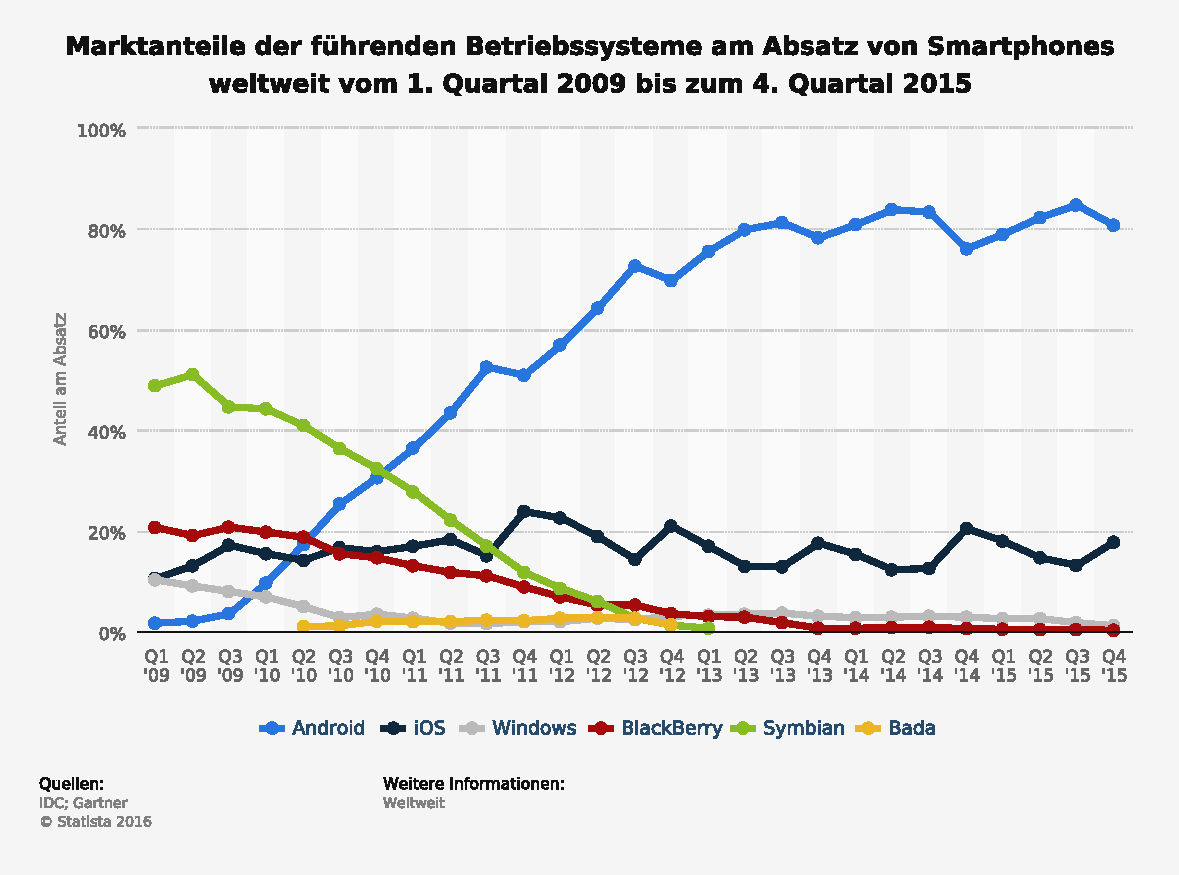
\includegraphics[width=\textwidth]{images/statistic_id73662_marktanteile-der-smartphone-betriebssysteme-am-absatz-weltweit-bis-q4-2015.pdf}
    \caption{Marktanteile der Smartphone Betriebssysteme am Absatz weltweit\cite{smartphonemarktanteil}}
    \label{fig:marktanteil}
\end{figure}


\subsection {Android NotificationManager}

Notifications sind die vom Android Betriebssystem vorgesehene Art und Weise, 
wie eine Applikation die Nutzerin über einen Vorfall aufmerksam macht, während die Applikation nicht im Vordergrund ist.
Dies kann zum Beispiel im Falle der Signal Messenger App eine eingetroffene SMS sein,
oder der erfolgreiche Abschluss eines Updates vom Google Play Store.
Eine gepostete Notification taucht im Allgemeinen zunächst als kleines Pop-up am oberen Bildschirmrand auf und wird dann in die 
Notification Area (siehe Abbildung \ref{fig:notificationarea}) abgelegt.
Durch das Öffnen des Notification Drawers (siehe Abbildung \ref{fig:notificationdrawer}) kann eine detailliertere Ansicht aller ungelesenen Notifications geöffnet werden und gelesene, beziehungsweise nicht relevante, Notifications entfernt werden 
\cite{androidnotification}.


\begin{figure}%[!htb]
\begin{minipage}{\textwidth}
\centering
  
\includegraphics[width=0.75\textwidth]{images/Screenshot_2016-03-25-14-34-00.png}
  \subcaption{Notification Area\cite{androidnotification}}
  \label{fig:notificationarea}
\end{minipage}
\vfill
\begin{minipage}{\textwidth}
\centering
  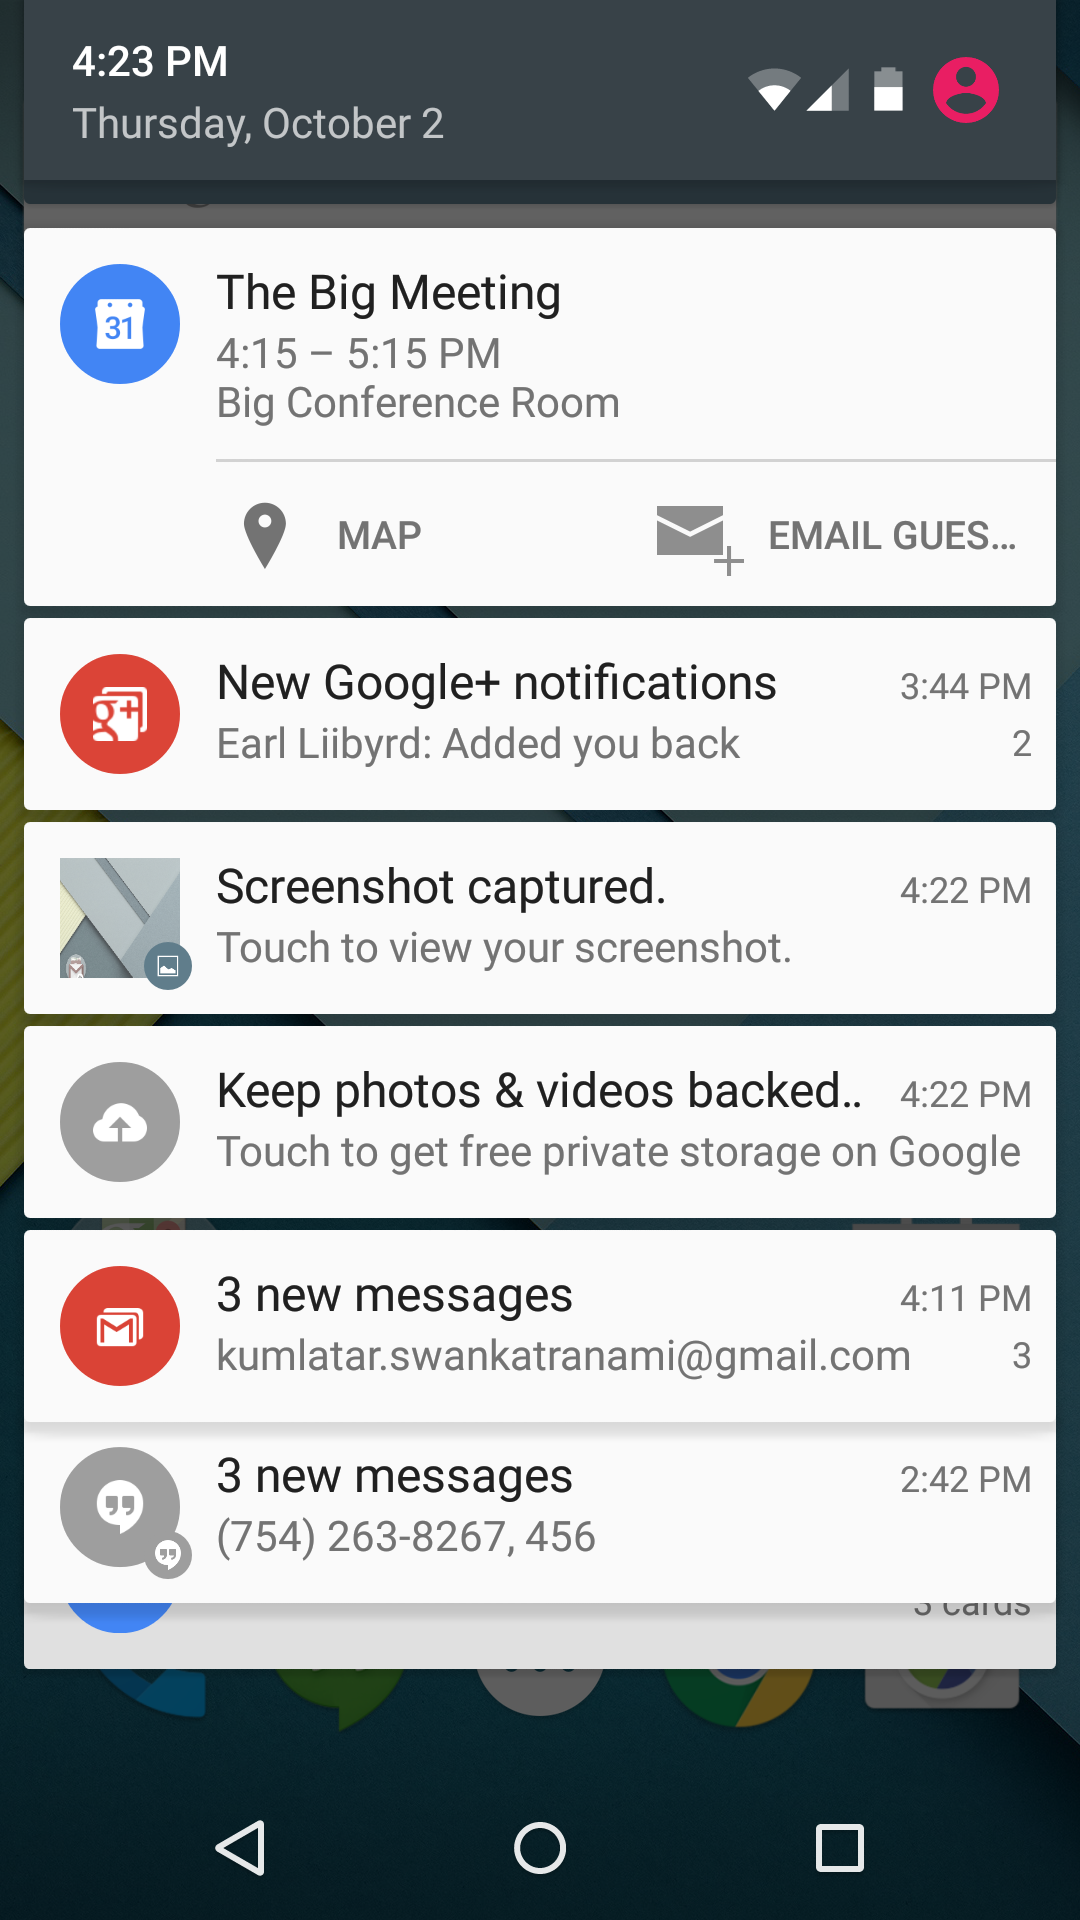
\includegraphics[width=0.5\textwidth]{images/notification_drawer.png}
  \subcaption{Notification Drawer\cite{androidnotification}}
  \label{fig:notificationdrawer}
\end{minipage}
\vspace{-2mm}
\caption{Notificationanzeige in Android}
\label{fig:notAndroid}
\end{figure}

Die Nutzerin kann einstellen, welche Apps Notifications senden dürfen und welche nicht.
So wird ein Spiel, das konstant auf sich selbst aufmerksam zu machen versucht, wahrscheinlich geblockt,
während dem E-Mail Client, der die Nutzerin auf neu angekommene E-Mails aufmerksam macht, diese Berechtigung erteilt wird.
Dementsprechend ist anzunehmen, dass die tatsächlich erhaltenen Notifications die Interessen der Nutzerin widerspiegeln.
\par

Der NotificationManager ist die Stelle im Android Betriebssystem, an der der Zugriff auf alle Notifications verwaltet wird und an der man mit ihnen interagieren kann.
Das beinhaltet beliebige Notifications zu erstellen oder gepostete Notifications zu löschen.
An den NotificationManager gebunden werden kann ein sogenannter NotificationListener, mit dem die Applikation alle an den NotificationManager geschickten Notifications lesen kann.
Dies beinhaltet unter anderem

\begin{description}
    \item [Package] Applikation, die die Notification gepostet hat
    \item [Notification Titel] Titel, oft der Absender der Nachricht
    \item [Ticker] Zusammenfassung der Notification für accessibility services
    \item [Text] Inhalt der Notification
\end{description}

Dies ist eine potenziell leicht zu missbrauchende Berechtigung, bei der Missbrauch katastrophalen Folgen haben kann.
Zum Schutz des Smartphones kann deshalb die Berechtigung nicht bei der Installation gegeben werden, sondern muss von Hand von der Nutzerin bestätigt werden. 


\subsection {Android UsageStatManager}

Der UsageStatManager ist eine Schnittstelle, die Zugang zu vom Betriebssystem gesammelten Daten
und Statistiken bezüglich der Nutzungshistorie des Geräts gibt \cite{androidusagestat}.
Die Methode \textbf{queryUsageStats(int intervalType, long beginTime, long endTime)} gibt eine Liste an UsageStats der verschiedenen Applikationen zurück.
Für jedes Element der Liste erhält man mit der Methode \textbf{getTotalTimeInForeground ()} die Zeit in Millisekunden,
die die App mit dem Package Namen aus \textbf{getPackageName ()} im Vordergrund war.
\par
Die \textbf{android.permission.PACKAGE\_USAGE\_STATS} Permission wird von der UsageStatManager API benötigt.
Diese ist ebenfalls eine missbrauchsanfällige privilegierte Berechtigung, die Applikationen zwar beantragen können, die aber nicht bei der Installation erteilt werden kann.
Sie muss von der Nutzerin von Hand bestätigt werden.


%% ==============================
\section{Verwandte Arbeiten}
%% ==============================
\label{ch:Grundlagen:sec:RelatedWork}

Auf dem Gebiet der Persönlichkeitsforschung wurden bereits einige Paper und Studien publiziert,
die das Feld thematisch mit Smartphonenutzungsdaten verknüpfen. 
Verschiedene Arbeiten verfolgen verschiedene Ansätze mit verschiedenen Persönlichkeitsmodellen und betrachten verschiedene Smartphone Features.
In diesem Kapitel sollen einige dieser Arbeiten betrachtet und Vor- und Nachteile der verwendeten Methoden abgewogen werden.

\section*{Personality and Self-Esteem as Predictors of Young People’s Technology Use}

In A. Ehrenbergs 2008 im "`CyberPsychology \& Behavior"' Journal erschienenen Artikel "'Personality and Self-Esteem as Predictors of Young People’s Technology Use"' \cite{ehrenberg2008personality}
wird das Ergebnis einer an 200 Universitätsstudentinnen, davon 146 weiblich und 54  männlich, durchgeführte Studie vorgestellt.
Die Probandinnen füllten sowohl einen 60 Fragen umfassenden NEO-FFI Fragebogen aus, als auch einen 25 Fragen umfassenden Fragebogen zur Bewertung des Selbstwertgefühls.
Dazu kam eine Liste an von der Nutzerin selbst geschätzten Zeitwerten, wie viele Minuten sie jeweils pro Tag mit (a) Telefonaten, (b) SMS und (c) Instant Messaging verbringe.
Abschließend sollten die Probandinnen Aussagen auf ihre Zustimmung hin bewerten, um einzuschätzen wie viel Suchtpotenzial von Technologien für sie ausgeht.
Die Studie fand einen starken Zusammenhang zwischen der Menge an Zeit, die mit diesen Technologien verbracht wird und dem persönlichen Suchtpotenzial.
Persönlichkeit und Selbstbewusstsein wurden als relativ schwache Indikatoren für die aufgewendeten Zeiten identifiziert.
\par
Die Wahl von Studentinnen als Zielgruppe ist aufgrund ihrer Rolle als Innovators und Early Adopters von neuen Technologien bei einer solchen Studie sehr zielführend.
Auch der Einsatz des Big Five Persönlichkeitsmodells als etablierter Standard, implementiert durch den NEO-FFI Fragebogen, ergänzt mit dem Wert für das Selbstwertgefühl, ist gut gewählt um eine Ground Truth zu bestimmen.
Im Gegensatz dazu steht die Wahl der Methodik zum Sammeln der Informationen bezüglich der Technologienutzung.
Einschätzungen von Nutzerinnen über das eigene Verhalten sind notorisch unpräzise und voreingenommen.
Auch die Wahl von "`Minuten mit X verbracht"' als (einziger) Messwert für Telefonanrufe, SMS und Instant Messaging ist fragwürdig und, abgesehen von Telefonaten, kein guter Indikator für die Intensität der Nutzung dieser Kommunikationswege.


\section*{Personality and Self reported Mobile Phone Use}

Sarah Butts Artikel "`Personality and self reported mobile phone use"', der im Jahr 2008 im "`Computers in Human Behavior"' Journal veröffentlicht wurde,
behandelt eine Studie, die versucht basierend auf den fünf Persönlichkeitsfacetten des Big Five Modells die Menge und Art der Mobiltelefonnutzung vorauszusagen.
Dazu berichteten 112 Versuchsprobandinnen, davon 78 weiblich und 54 männlich, zwischen 18 und 59 Jahren ihr persönliches Verhalten bezüglich Mobiltelefonen.
Außerdem füllten diese Versuchsprobandinnen den NEO-FFI Persönlichkeitsfragebogen und das Copperfield Self-Esteem Inventory aus.
Der Bericht der Mobiltelefonnutzung beinhaltete folgende Fragen: Zeit aufgewendet für Anrufe, für SMS, für Spiele auf dem Mobiltelefon und für das Ändern von Klingelton beziehungsweise Wallpaper.
Außerdem eine Schätzung wie viele Anrufe getätigt und empfangen wurden, wie viele der ausgehenden Anrufe persönlicher und wie viele geschäftlicher Natur waren und wie viele der eingehenden Anrufe als erwünscht oder unerwünscht eingeschätzt werden.
Zusätzlich wurde erfragt ob SMS oder Anrufe präferiert werden, wie viel Interesse an neuen Features von Mobiltelefonen besteht und wie lange die Probandin bereits ein Mobiltelefon besitzt.
Die Studie ergab, dass extrovertierte Individuen tendenziell mehr Zeit mit Anrufen und dem Ändern von Klingelton und Wallpaper verbringen.
\par
Wie schon bei der vorangehenden Studie benutzt auch diese Studie den NEO-FFI Fragebogen und ergänzt diesen mit einem Wert für das Selbstwertgefühl der Probandin, was für die Validität dieses Verfahrens spricht.
Die erhobenen Daten sind bedeutend besser gewählt als in der vorangehenden Studie, da sie nicht nur die verbrachte Zeit, sondern auch die Anzahl, den Willen der Probandin und deren Präferenz bezüglich SMS oder Anruf erfragt.
Jedoch verlässt sich diese Studie ebenfalls auf Selbsteinschätzungen, was bei Fragen wie zum Beispiel nach der Präferenz zwischen Anruf und SMS sicher sinnvoll ist, aber bei Werten wie Anrufdauer oder Anzahl der Anrufe notorisch unpräzise ist.
Ebenfalls bemerkenswert ist, dass eine Studie, die im Jahr 2008 durchgeführt wurde, also zwei Jahre nach dem Release des ersten Apple iPhones und während des bereits beginnenden Siegeszug der Smartphones, die Features, die Smartphones ausmachen, nicht mit in Betracht zieht.

\section*{The Impact of Personality Traits on Smartphone Ownership and Use}

Die von W. Lane et al 2011 veröffentliche Studie "`The Impact of Personality Traits on Smartphone Ownership and Use"' untersucht den Effekt der Ausprägung der verschiedenen Big Five Persönlichkeitsfacetten.
Von 312 Teilnehmerinnen, davon 60\% weiblich und 40\% männlich, im Alter zwischen 17 und 88 Jahren wurden Werte für die verschiedenen Persönlichkeitsfacetten des Big Five Modells ermittelt
Darüber hinaus sollten die Teilnehmerinnen sechs Funktionen von Smartphones auf einer Skala von 1 bis 5 bezüglich ihrer Wichtigkeit bewerten.
Diese sechs Funktionen waren Anrufe, SMS, Internet, E-Mail, Musik und Spiele.
Zur Bestimmung der Facettenwerte wurde John's (1991) Big Five Personality Inventory aufgrund seiner geringen Komplexität und schnellen Durchführbarkeit gewählt.
Die Studie ergab, dass Probandinnen, die höher auf der Extraversionsskala lagen, eher Smartphones besaßen und benutzen und relativ viel Wert auf die SMS Funktion des Smartphones legen. 
\par
Positiv bei Lanes Studie ist die große Anzahl und die breite Altersspanne der Testprobandinnen anzumerken.
Kritisch zu sehen ist die Wahl der Methode zum Bestimmen der Persönlichkeit der einzelnen Probandinnen und die sehr geringe Tiefe der Fragen zur Benutzung des Smartphones.


\section*{Who’s Who with Big-Five: Analyzing and Classifying Personality Traits with Smartphones}

G. Chittaranjan et al stellen in ihrem Paper "`Who’s Who with Big-Five: Analyzing and Classifying Personality Traits with Smartphones"' ihre acht-monatige Studie an 83 Individuen vor.
Im Laufe dieser acht Monate werden auf den Nokia N95 Smartphones \ref{nokia} der Probanden eine breite Menge an Daten bezüglich Anrufen, SMS, Applikationen und Bluetooth gesammelt, 
die dann mit den per NEO-FFI festgestellten Facettenwerten verglichen werden.
Basierend darauf haben die Autoren eine automatisierte Methode entwickelt, die den Persönlichkeitstyp anhand von Smartphone Daten erkennt.
Diese Methode erzielt eine Genauigkeit von 75,9\%.
\par
Die hier vorgestellte Studie überzeugt durch ihren großen Umfang, sowohl was die Studiendauer angeht, als auch die breite Palette an direkt vom Smartphone gesammelten Daten.
Dadurch, dass die Daten direkt auf dem Gerät gesammelt werden, sind diese verlässlicher und präziser als die der bisher aufgeführten Arbeiten.
Die Wahl des NEO-FFI Fragebogens ist solide.
Die Auswahl der gesammelten Daten bezüglich der Applikationsnutzung ist potenziell fraglich, da nur die Anzahl an Nutzungen und nicht die Länge oder Intensität in Betracht gezogen werden.
Aus heutiger Sicht entsprechen die Eigenschaften des Nokia N95 nicht mehr dem, was von einem gängigen Smartphone erwartet wird.
Es verfügt weder über einen Touchscreen noch über Multitasking.
%Auch die ist Wahl des Nokia N95 als Zielgerät der Studie ist, zumindest aus heutiger Sicht, nicht vernünftig, da Nokias Versuche sich auf dem Smartphone Markt zu etablieren nicht von Erfolg gekrönt waren.
%Der frühere Marktführer stellte nicht lang nach Veröffentlichung der Studie die eigene Entwicklung des Symbian Betriebssystem ein\cite{nokiaabort} und verkaufte nach einigen weiteren Fehlschlägen seine Mobiltelefonsparte an Microsoft im Jahr 2014\cite{nokiasell}.  


\section*{StudentLife: Assessing Mental Health, Academic Performance and Behavioral Trends of College Students using Smartphones}

Die von R. Wang et al durchgeführte Studie "`StudentLife: Assessing Mental Health, Academic Performance and Behavioral Trends of College Students using Smartphones"'
betrachtet den Einfluss von Arbeitsbelastung auf Stress, Schlaf, Aktivitäten, Laune, Geselligkeit, mentale Gesundheit und akademische Leistung.
Dies geschieht anhand von 38 männlichen und 10 weiblichen Computer Science Studentinnen einer Klasse am Dartmouth College in den Vereinigten Staaten über den Verlauf eines Terms (10 Wochen).
Dazu werden auf dem Smartphone gesammelte Daten mit vor und nach dem Term ausgefüllten gesundheitlichen und psychologischen Gutachten und den akademischen Ergebnissen der Studentinnen zusammen ausgewertet.
Die auf den Smartphones der Studentinnen installierte Applikation klassifiziert Aktivität, fordert die Studentinnen auf kurze Assessments ihrer aktuellen Situation zu geben und überprüft durch Aufzeichnen der Umgebungsgeräusche und Analyse auf Konversationsaktivität die Geselligkeit der Nutzerin.
Das Ergebnis der Studie ist die Indentifikation eines Dartmouth Lebenszyklus, wonach das Stresslevel und Arbeitsbelastung mit fortschreitender Zeit im Term steigt und Schlaf, Geselligkeit und Aktivitäten dafür nachlassen.
\par
Wangs Studie zeugt von beeindruckendem Aufwand in vielen Aspekten. 
Die gesammelten Daten enthalten eine große Reichweite an Informationen, die unter anderem auch nur durch sehr exklusive Zugriffe, wie zum Beispiel intime Kenntnisse der Dartmouth Campus W-LAN Infrastruktur oder Zugang zu den Noten der Studienteilnehmerinnen, zu erreichen sind.
Auch positiv ist, dass viele dieser Daten tatsächlich objektive sind und nicht durch Selbsteinschätzung der Probandinnen generiert wurden.
Die komplette Auflösung der Privatsphäre der teilnehmenden Studentinnen, unter anderem durch das konstante Mitschneiden von Ton, ist für eine Studie im Rahmen einer Bachelorarbeit nicht denkbar. 
Auch sind viele der betrachteten Aspekte nicht mit den Resourcen einer Bachelorarbeit nicht auszuwerten.



\begin{figure}[h]
    \centering
    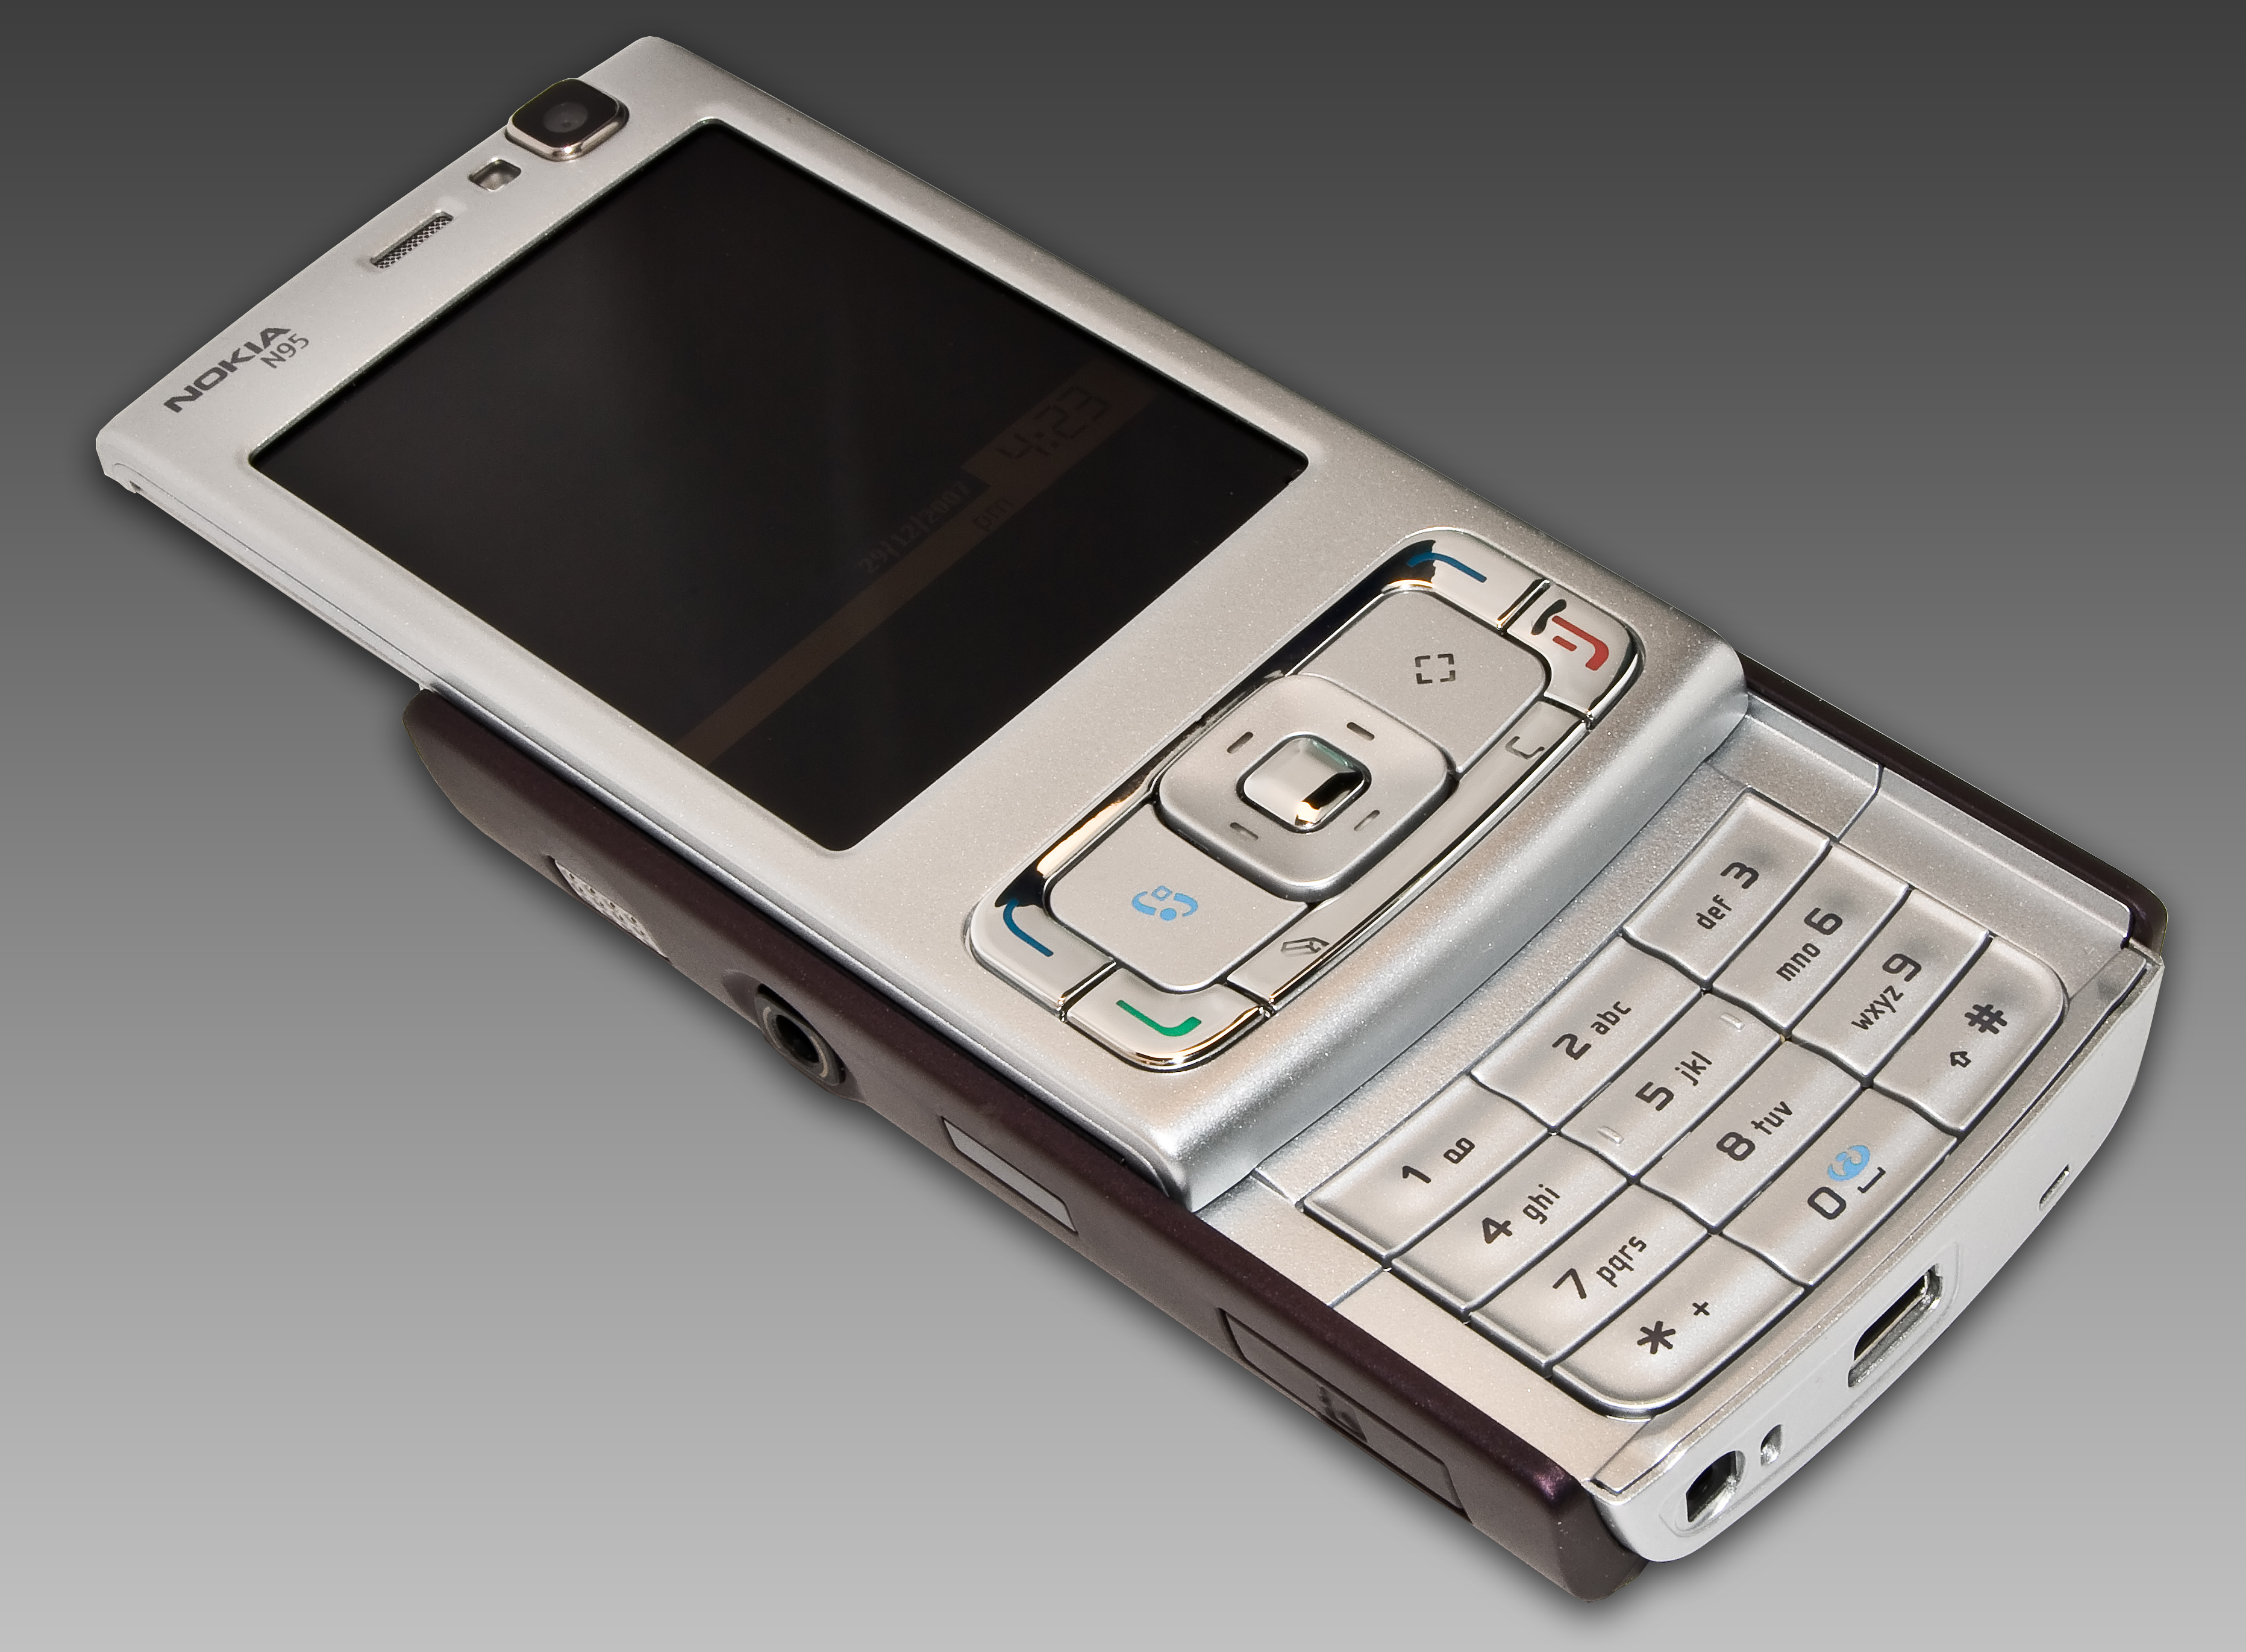
\includegraphics[width=0.5\textwidth]{images/N95_Front-slide-open}
    \caption{Nokia N95\cite{nokiaPhone}}
    \label{nokia}
\end{figure}

\ignore{ Notizen: \\

Work 1: "`StudentLife: Assessing Mental Health, Academic Performance and Behavioral Trends of College Students using Smartphones"'
48 Computer science students. 10 Wochen (ein Term)
Betrachtet Workload -> Stress, sleep, mood, \textbf{sociability}, activity, mental wellbeing und academic preformance.
Benutzt android.
Backup über wifi jedes mal wenn das handy geladen wird
"`During the collection phase, students were asked to respond to various EMA questions as they use their phones"'
Students werden per email benachrichtigt wenn die Daten ausbleiben.
The StudentLife app automatically infers activity (stationary, walking, running, driving, cycling), sleep duration, and sociability (i.e., the number of independent conservations and their durations). The app also collects accelerometer, proximity, audio, light sensor readings, location, colocation, and application usage.
Das handy schneidet ton mit und detectet conversationen.
A series of entry health and psycholog- ical baseline surveys are administered 
During the exit stage, we administered an exit survey, interview and the same set of be- havioral and health surveys
2014
\par

Work 2: "`Who’s Who with Big-Five: Analyzing and Classifying Personality Traits with Smartphones"'
83 french speaking switzerlanders over 8 months
Shown: aggregated features obtained from smartphone usage data can be indicators of the Big-Five personality traits
automatic method to infer the personality type of a user based on cellphone usage
75.9\% accuracy
Nokia n95 phone (bild!)
NEO FFI
gesammelte Features: calls (Call Logs), SMS (SMS Logs), bluetooth scans (BT Logs ), and application usage (App Logs ) (Nur Anzahl von öffnen, nicht zeit).
2011

\par
work 3: "`The Impact of Personality Traits on Smartphone Ownership and Use"'
312 participants
This study directly tests the effect of the "Big Five" personality traits on smartphone ownership and use.
We found that extraverted individuals were more likely to own a smartphone. Also, extraverts reported a greater importance on the texting function of smartphones
Age ranged from 18 to 77 years with a median age of 41 and a mean age of 40.
Respondents who owned a smartphone were then asked to rate on a five-point scale (1, not important at all, to 5, very important) the importance of six smartphone functions: phone calls, texting, internet, e-mail, music, and games. 
We measured personality with John’s (1991) Big Five Personality Inventory
2011

\par
Work 4: "`Personality and Self-Esteem as Predictors of Young People’s Technology Use"'
Participants were 200 university students (146 females, 54males)
Personality: The 60-item NEO FFI Personality Inventory + The 25-item Coopersmith Self-Esteem Inventory Adult Form
Self report: Time Spend on calls, sms and IM, and addictive tendencies towards those. 
2008

\par
work 5: "`Personality and self reported mobile phone use"'
112 participants in this study (78 females, 34 males). Age ranged from 18 to 59 years.
The Coopersmith self-esteem inventory
NEO-FF
selfreport- Mobile phone use survey}



%%% Local Variables: 
%%% mode: latex
%%% TeX-master: "diplarb"
%%% End: 
  % Grundlagen
%% analyse.tex
%% $Id: analyse.tex 28 2007-01-18 16:31:32Z bless $

\chapter{Analyse}
\label{ch:Analyse}
%% ==============================

Nach der Klarstellung der grundlegenden Begrifflichkeiten im vorhergehenden Kapitel
sollen nun die Anforderungen und Limitationen einer Studie festgestellt werden, die den
Zusammenhang zwischen der Nutzung von Social Media, Instant Messaging und der Geselligkeit
von Nutzern untersuchen soll. 
Dazu werden auch bereits existierende Lösungsansätze betrachtet. 

%% ==============================
\section{Anforderungen}
%% ==============================
\label{ch:Analyse:sec:Anforderungen}

%Anforderungen und Randbedingungen\index{Randbedingungen} \ldots

Für die Untersuchung des Zusammenhanges werden zwei Datensätze benötigt.
Auf der einen Seite ein wie auch immer gearteter Wert für die Geselligkeit der Probandin. 
Dem gegenüberstehend wird ein Datensatz, der Informationen über das Nutzungsverhalten ebenjener Probandin enthält, benötigt.
\par

\subsection{Geselligkeit}

Der Duden definiert Geselligkeit als Ungezwungenheit beim Umgang beziehungsweise dem Verkehr mit anderen Menschen und der Gesellschaft \cite{dudengesell}.
Ein solch abstraktes Konzept kann für verschiedene Menschen sehr verschiedene Formen annehmen.
Trotzdem muss für die wissenschaftliche Auseinandersetzung mit dem Thema dieses Konzept quantifiziert betrachtet werden.
Eine valides Modell dieses Problem muss durch ein standartisiertes Verfahren einen im Optimalfall numerischen Wert für diese Ungezwungenheit liefern. 
\par

Ein solches Modell, das zum Beispiel auf auch im Paper "`Who’s Who with Big-Five: Analyzing and Classifying Personality Traits with Smartphones"'\cite{chittaranjan2011s} genutzt wird, ist das Big Five Modell.
Dort ist Geselligkeit eine Unterfacette der Extraversion.
Eine oft genutzte Option um in diesem Modell numerische Werte für die verschieden Facetten und Unterfacetten zu erschließen ist eine Familie von Selbstbeurteilungsfragenbogen,
die zum Beispiel auch in T. Correa's "`Who interacts on the Web?: The intersection of users’ personality and social media use"' \cite{butt2008personality} genutzt wird.
Zu dieser Familie gehören unter anderem der ursprünglichen NEO-Inventory-  (1978), der NEO-Personality Inventory- (1985) und der NEO-Five Factory Inventory-Fragenbogen.
Im Rahmen dieser Arbeit wird der auf dem NEO-PI basierende überarbeitete NEO-Personality Inventory-Revised-Fragebogen in der Version von 2003 benutzt\cite{neopir2003}
um der Extraversion und der Geselligkeit der einzelnen Testprobandinnen einen numerischen Wert zuzuordnen.

Die Entscheidung für den NEO-PI-R liegt nahe: 
Er ist gemeinsaml mit dem NEO-FFI der aktuellste Fragebogen dieser Familie und liefert mit seinen insgesamt 241 Fragen, davon zumindest 48 Fragen auf Extraversion bezogen,
einen nuancierterer Blick auf die Persönlichkeit der durchführenden Person als der NEO-FFI, der insgesamt nur 60 Fragen hat und dementsprechend nur mit 12 Fragen zur Extraversion aufwartet.



\subsection{Nutzungsdaten}

Von besonderer Relevanz für das Sammeln der Nutzungsdaten ist es festzulegen welche Daten zur Verfügung stehen, welche relevant sind und welche potenziell trotzdem nicht gesammelt werden sollten.
Für diese Arbeit werden keine Nutzerdaten von physische Sensoren in Betracht gezogen, sondern nur die Interaktion mit dem Smartphone als Kommunikationsgerät.
Zu diesem Zweck interagiert die Applikation mit Schnittstellen des Android Betriebssystems.
Dies vermeidet das potenzielle Problem von unterschiedlicher Hardware und sorgt dafür, dass die Nutzungsdaten von allen Testprobanden vergleichbar bleiben.
Zudem vermeidet dies übermäßige Mehrbelastung der Akkuleistung der Smartphones, auf denen die Applikation installiert wird.
Allgemein ist es wünschenswert die Belastung der Resourcen auf den Zielgeräten so gering wie möglich zu halten.
\par

Eine der stärksten Limitation für die Daten, die die Applikation sammeln kann, kommt von der Natur der zu betrachtenden Daten.
Zum einen begrenzt das Android Betriebssystem selbst die Informationen zu denen eine Applikation, selbst eine die vom Nutzer mit potenziell jeder Berechtigung ausgestattet wurde, Zugang hat.
Dies geschieht aus Datenschutz gründen, da manche Applikationen im Play Store mehr Berechtigungen einfordern als sie für ihr Funktionieren benötigen würden.
Zum anderen sind die Kommunikationsapplikationen, die die Testprobandin nutzt von unabhängigen Drittentwicklern entworfen worden.
Einige Wenige von diesen stellen in ganz speziellen Fällen, zum Beispiel Twitter\cite{twitterapi}, zwar eine API zur Verfügung, die meisten hüten ihre Daten aber.
Folglich können nur Daten gesammelt werden, die entweder frei zugänglich sind, oder solche, zu denen die Nutzerin Applikationen Zugriff erlauben kann.
Beispiele hierfür sind zum Beispiel die Call logs in denen Android, für alle Apps mit der Berechtigung \textbf{android.permission.READ\_CALL\_LOG}, die vergangenen Anrufe abspeichert.
\par

In diesem Kontext ist das Android API Ziellevel der Applikation von großer Bedeutung.
Wie bei Smartphone Betriebssystemen üblich wird das Android Betriebssystem konstant weiterentwickelt und neue Versionen davon werden ausgeliefert.
Potenzielle Änderungen an Systemschnittstellen werden dabei durch die verschiedenen API Levels dokumentiert, auf die sich installierte Applikationen berufen können.
Die aktuellste Version von Android ist Android 6.0, oder auch Android Marshmallow.
Diese wird repräsentiert durch das API Level 23.
Da nicht alle Geräte aber die steigenden Anforderungen der neueren Android Versionen erfüllen, 
und manche Nutzer neu herauskommende Updates selbst dann nicht installieren, wenn ihr Gerät sie unterstützt, 
sei es auf Grund von Faulheit, Unwissenheit oder Bequemlichkeit, sind auf vielen Smartphones ältere Android Versionen vertreten.
Eine Übersicht über die Verteilung der Android Versionen sieht man im Diagramm \ref{fig:androidplatformdistr}.
Mit 36.1\% ist Android 5, beziehungsweise Android Lollipop die am weitesten verbreitetste Version,
gefolgt von Android 4.4 (Kitkat) mit 34.3\% und Android 4.0-4.3 (Jellybean) mit 22.3\%\cite{androiddistr}.
Für die Entwicklung der Applikation wird Android API level 21, entspricht Android 5.0, als Ziellevel bestimmt, da es einige relevante Schnittstellen hinzufügt die bei niedrigeren Leveln noch nicht existieren, aber auch eine breit genuge Userbasis hat, um ausreichend viele Probanden zu finden.


\begin{figure}[h]
    \centering
    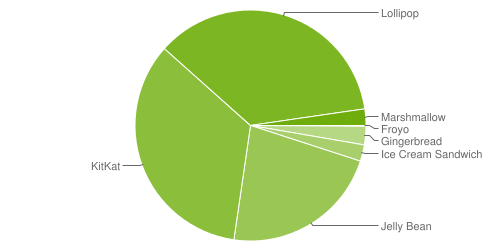
\includegraphics{images/chart.png}
    \caption{Android Platform Distribution\cite{androiddistr}}
    \label{fig:androidplatformdistr}
\end{figure}

Auch die Empfindungen potenzieller Testprobandinnen müssen in Betracht gezogen werden:
Während die Anzahl an Anrufen in den vergangenen 14 Tagen von vielen als Unkritisch betrachtet werden würde, so gibt es sicher eine Menge Menschen, 
die eine Liste von Telefongesprächen inklusive Zeitpunkt und Rufnummer des Partners als zu tiefen Eingriff wahrnehmen würden.
Ziel muss es hier sein bezüglich der Geselligkeit aussagekräftige Datenpunkte zu wählen, 
die aber dennoch nicht das grundlegende Bedürfnis nach Privatsphäre der Probandinnen verletzt.


\subsection{Datenschutz}

Die Daten mit denen im Rahmen dieser Studie gearbeitet werden sind sehr sensibler Natur.
Dementsprechend muss sicher gestellt werden, dass sowohl die Anonymität der einzelnen Probandinnen gewahrt bleibt,
als auch dass die Daten nicht den Rahmen der Studie verlassen.
Dazu werden die erhobenen Daten pseudonymisiert, das heißt zur Indenfikation der Zugehörigkeit von Fragebogen und erhobenen Daten wird nicht der Name der Versuchsteilnehmerin genutzt sondern ein frei gewähltes Pseudonym.
Außerdem werden keinerlei persönlichkeitsbezogene Daten im Klartext gespeichert.
Weder Telefonnummern, noch Absender oder Nachrichteninhalte werden in Klartext geloggt.
Stattdessen werden die relevanten Features der Daten in anderer Form abgespeichert:
Unter anderem Anzahl verschiedener Telefonnummern, durch Hashen unkenntlich gemachte Nachrichtenabsender und Ersetzen der Nachrichtentexte durch die Anzahl der Zeichen in der Nachricht.
Dennoch wird, wie bei allen Studien dieser Art, die am TECO durchgeführt werden,
eine unterschriebene Einwilligungserklärung seitens der Probandin benötigt.
In dieser wird das Einverständnis der Probandin bezüglich der Aufzeichnung, Speicherung und Verarbeitung zugesichert.
\ignore{siehe Anhang, adde anhang?}
\par



%% ==============================
\section{Existierende Lösungsansätze}
%% ==============================
\label{ch:Analyse:sec:RelatedWork}

Hier kommt eine ausführliche Diskussion
von "`Related Work"'.

Bla fasel\ldots

%% ==============================
\section{Zusammenfassung}
%% ==============================
\label{ch:Analyse:sec:zusammenfassung}

Für diese Arbeit sind die Wahl eines sinnvollen Modells für die Messung der Geselligkeit eines Menschen 
und die Auswahl von relevanten und verfügbaren Daten die Mittels der Android Applikation gesammelt werden sollen von zentraler Bedeutung.
Für die Applikation ist außerdem wichtig, dass sie so leichtgewichtig wie möglich ist, 
sowohl was die Bedienung durch die Probandinnen angeht, als auch den Stromverbrauch und die Belastung auf Speicher und Prozessor angeht.
Alle erhobenen Daten müssen im Kontext von Datenschutz und Schutz der Privatssphäre betrachtet und überdacht werden.

%%% Local Variables: 
%%% mode: latex
%%% TeX-master: "diplarb"
%%% End: 
     % Analyse
%% entwurf.tex
%% $Id: entwurf.tex 28 2007-01-18 16:31:32Z bless $
%%

\chapter{Entwurf}
\label{ch:Entwurf}
%% ==============================

Für das Aufzeichnen, der für die Studie relevanten Daten wird eine auf dem Smartphone der Probandin installierte Android Applikation benötigt. 
Dieses Kapitel beschäftigt sich mit dem Entwurf dieses App und setzt sich mit dem Zugriff verschiedener Datenquellen auseinander.
Eine grobe Skizze des Systems ist in Abbildung \ref{skizze} zu sehen.
Der Entwurf soll darauf abzielen, der Nutzerin möglichst wenig aufzufallen, um ihr Verhalten nicht zu beeinflussen.
Das Ziel soll sein, keinerlei Interaktion abgesehen von der Installation und dem Export der Daten zu benötigen. 
\par

Die App zur Studie wurde für Geräte mit mindestens Android 5.0 "`Lollipop"', das entspricht dem API Level 21, entworfen.
Das heißt, dass aufgrund der Rückwärtskompabilität auch alle neueren Geräte in der Lage sind die Applikation auszuführen.
\par

%%Die Entscheidung als Minimal API Level 21 zu wählen geht war notwendig, da mit diesem die UsageStatManager Schnittstelle für Applikationen zum Android Betriebssystem hinzugefügt wurde.
%%Von anderen Aspekten der Applikation benötigte API Levels waren:

Die Entwurfsentscheidung über das zu nutzende API Level ist immer eine Abwägung;
Auf der einen Seite steht das niedrigere API Level, das wie im Grundlagenkapitel \ref{ch:Grundlagen} beschrieben, 
eine breitere Menge an potenziellen Testprobandinnen eröffnet.
Andererseits haben höhere API Level oft viele Verbesserungen und neue Schnittstellen mit denen Entwickler mehr Funktionalität erreichen können.
\par
Die Entscheidung für das relativ aktuelle API Level 21 ist motiviert davon, 
dass der potenzielle Pool von Testprobandinnen im Umfeld der Informatik oft über aktuellere Smartphones und Android Versionen verfügt
und dass mit Level 21 einige Neuerungen im Bereich der Aufzeichnung von Applikationsaktivität hinzugefügt wurden.

Untermauert wird dies von der bereits im vorangehenden Kapitel vorgestellten Statistik \ref{fig:androidplatformdistr}  von Google\cite{androiddistr}, 
die Android 5.0 "`Lollipop"' mit 36.1\% als die meistgenutzte Version des Android Betriebssystems.

\par

%TODO: Systemskizze.
\begin{figure}[h]
    \centering
    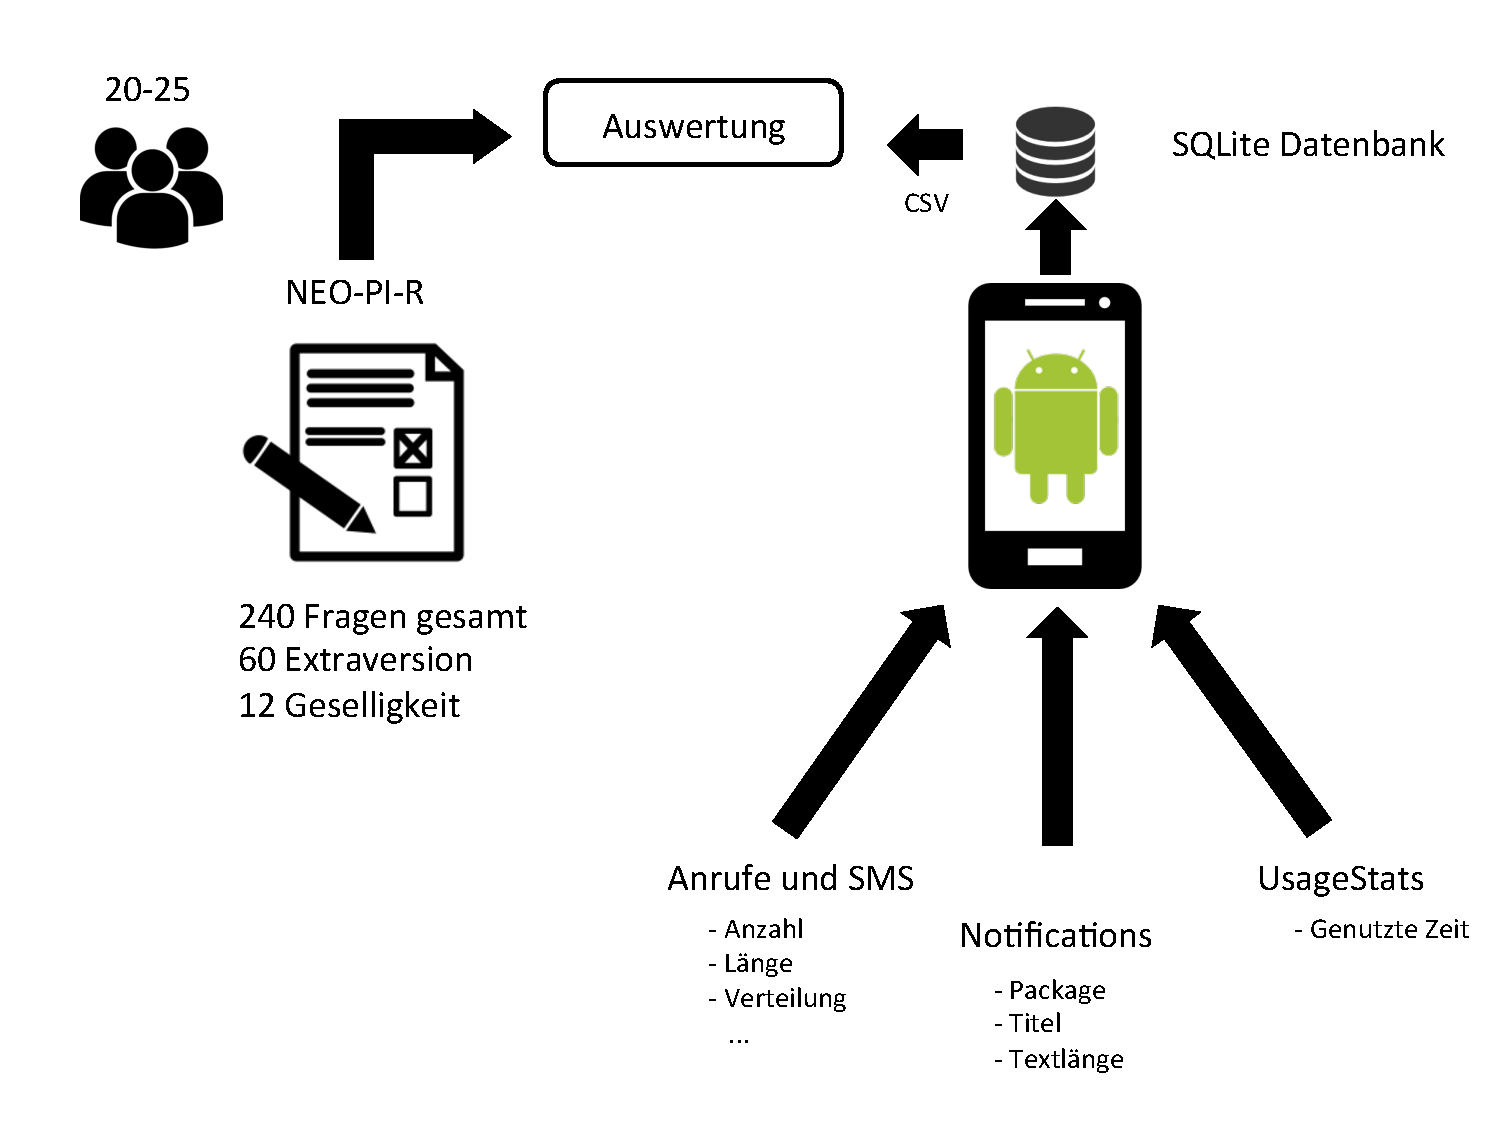
\includegraphics[width=\textwidth]{images/skizze.pdf}
    \caption{Systemskizze}
    \label{skizze}
\end{figure}


\section{Datenquellen}

%Das Nutzungsverhalten der Studienteilnehmerinnen soll mit einer Android Applikation aufgezeichnet werden.
%Die Applikation soll mit so wenig Nutzerinteraktion wie möglich auskommen.
Für das Aufzeichnen des Nutzerverhaltens werden drei beziehungsweise vier verschiedene Datenquellen betrachtet.
\par

\subsection{Call und Message Log}
Zunächst werden die konventionellen Kommunikationsmöglichkeiten eines normalen Mobiltelefons betrachtet.
Daten zu Anrufen und Kurznachrichten (SMS) lassen sich in Android mit Zugang zum \emph{Call Log} und zum \emph{Message Log} auslesen.
Die Berechtigungen dafür können von der Nutzerin bei der Installation erteilt werden und müssen nicht nocheinmal bestätigt werden.
Für das Sammeln dieser Daten muss nicht aktiv das Verhalten der Nutzerin geloggt werden und es muss auch keine Datenbank dazu angelegt werden,
da das Android Betriebssystem dies bereits erledigt.
Es genügt beim finalen Abgeben der Daten auf die Call und Message Logs zuzugreifen und die relevanten Daten auszulesen, da man den Abfragezeitraum beliebig wählen kann.
Um ein aussagekräftiges Ergebniss zu erhalten ist die Wahl der relevanten Daten, die untersucht werden, von entscheidender Bedeutung. 
Aus diesem Grund wurden für diese Arbeit verschiedene Ansätze der Wahl der zu betrachtenden Features in Betracht gezogen. 
Dabei verspricht der Ansatz aus \cite{chittaranjan2011s} für unsere Zwecke auf Grund seiner breiten Fächerung die besten Resultate.
\par

%\subsection{Call Log}
Dementsprechend wurden folgende für diese Arbeit interessanten Features aus dem Call Log extrahiert:

\begin{itemize}
    \item Anzahl Anrufe gesamt
    \begin{itemize}
        \item Anzahl Anrufe ausgehend
        \item Anzahl Anrufe eingehend
        \item Anzahl Anrufe verpasst
    \end{itemize}

    \item Anrufdauer gesamt
    \begin{itemize}
        \item Dauer Anrufe ausgehend gesamt
        \item Dauer Anrufe eingehend gesamt
    \end{itemize}

    \item Durschnittliche Dauer gesamt
    \begin{itemize}
        \item Durchnittliche Dauer Anrufe ausgehend
        \item Durchnittliche Dauer Anrufe eingehend
    \end{itemize}

    \item Unique Anrufpartner
    \item Maximale Anzahl Anrufe mit einem Partner

\end{itemize}

%\subsection{Message Log}
Analog zum Call Log wurden folgende Features aus dem Message Log extrahiert:

\begin{itemize}
    \item Anzahl SMS gesamt
    \begin{itemize}
        \item Anzahl SMS gesendet
        \item Anzahl SMS empfangen
    \end{itemize}

    \item SMS Zeichenanzahl gesamt
    \begin{itemize}
        \item SMS Zeichenanzahl gesendet gesamt
        \item SMS Zeichenanzahl empfangen gesamt
    \end{itemize}

    \item Durchschnittliche SMS Zeichenanzahl gesamt
    \begin{itemize}
        \item Durchschnittliche SMS Zeichenanzahl gesendet
        \item Durchschnittliche SMS Zeichenanzahl empfangen
    \end{itemize}

\end{itemize}


\subsection{Notifications}


\ignore{todo: refereces}
Über den im Grundlagenkapitel bereits vorgestellten NotificationManager beziehungsweise einen NotificationListenerService kann auf dem Gerät der Nutzerin eine SQLite Datenbank angelegt werden,
in die alle während dem Studienzeitraum der Nutzerin gezeigten Notifications gespeichert werden.
Die Spalten der SQLite Datenbank sind die Folgenden:
\begin{description}
    \item ["`\_id"'] fortlaufende Indentifikationsnummer
    \item ["`notificationEntry"'] Package der Applikation von der die Notification gepostet wurde
    \item ["`titleHashed"'] Gehashter Titel der Notification, Bei Nachrichten oft der Absender
    \item ["`textLength"'] Anzahl Zeichen im Text der Notification
    \item ["`date"'] Zeitpunkt, an dem die Notification gepostet wurde
\end{description}

Im Sinne des Schutzes der Privatsphäre beinhalten diese Einträge nicht exakt den Inhalt der Notification, sondern so anonymisiert, dass die für die Studie relevante Information erhalten bleibt.
So wird der Titel der Notification mit dem SHA-1 Hash\cite{sha1def} gehasht.
SHA-1 ist eine 1995 von US Amerikanischen Nachrichtendienst NSA veröffentlichte kryptographische Hashfunktion\cite{sha1proposal}.
Dies führt dazu, dass für die Auswertung der Studie zwar zwischen zwei verschiedenen Absendern von Nachrichten unterschieden werden kann, diese aber nicht frei zu erkennen sind.
Ebenso speichert die Applikation für die Studie nur die Länge der erhaltenen Nachrichten und nicht deren Inhalt, da dies ein sehr harter Eingriff in die Privatssphäre wäre.
Der Zeitpunkt wird im Datenformat Millisekunden seit Epoch angegeben.


\subsection{UsageStats}

Über den im Android API Level 21 eingeführten UsageStatsManager ist es möglich 
auf die vom Android Betriebssystem selbst gesammelten Daten bezüglich der Zeit aller Applikationen im Vordergrund zuzugreifen.


TODO: MEhr UsageStats + Auswahl App + Statistik

\subsection{Auswahl Applikationen}

Um vom Umfang der Arbeit im Rahmen einer Bachelorarbeit zu bleiben und gleichzeitig nicht einen größeren Eingriff in die Privatsphäre der Probandin als nötig zu tätigen,
ist es notwendig, sich auf eine bestimmte Menge von Applikationen zu begrenzen, deren Notifications und UsageStats gesammelt werden sollen.

Hierzu wurden folgende Applikationen ausgewählt:
\begin{description}
  \item [Google Hangouts] Crossplattform Kommunikationsdienst von Google. Auf aktuellen Android Smartphones vorinstalliert.
  \item [Whatsapp] Crossplattform Instant Messaging Client. Mit über einer Milliarde Nutzer die meistgenutzte Messaging Application\cite{whatsappuser}.
  \item [Facebook App] Mobile Applikation des größten und aktivsten Social Networks mit über einer Milliarde aktiver Nutzer pro Tag\cite{facebookuser}.
  \item [Facebook Messenger] Dedizierte Messenger Applikation von Facebook.
  \item [Skype] Dedizierte VoIP und Messaging Applikation zu Microsofts Skype mit über 600 Millionen Nutzern\cite{skypeuser}.
  \item [Telegram] Crossplattform Kommunikationsdienst, das sich durch verschiedene Sicherheitsoptionen von seiner Konkurrenz abhebt. Über 100 Millionen Nutzer\cite{telegramuser}.
  \item [Twitter] Social Microblogging Service mit 300 Millionen aktiven Nutzern. Aufgrund der offenen API gibt es verschiedene Twitter Apps, von denen die größten betrachtet werden:
  \begin{itemize}
      \item Offizielle Twitter App
      \item Carbon for Twitter
      \item Plume for Twitter
      \item Talon for Twitter
  \end{itemize}
\end{description}




%% ==============================
\section{Zusammenfassung}
%% ==============================
\label{ch:Entwurf:sec:zusammenfassung}

Die Studie, die im Rahmen dieser Arbeit durchgeführt wird, untersucht zwei Datenpunkte.
Zum einen die von der Applikation gesammelten Daten zum Nutzungsverhalten von zehn bestimmten Social Media und Instant Messaging Applikationen
und zum anderen die zu der Nutzerin zugeordneten Extraversions-, beziehungsweise Geselligkeitswerte aus einem Persönlichkeitstest.
Als für das Einschätzen des Nutzerverhaltens relevante Smartphonedaten wurde einerseits die Häufigkeit, Länge und Verteilung von  Anrufen und SMS bewertet,
als auch die Notifications und UsageStat von zehn Kommunikations- und Social Media Applikationen.
Dabei wird besonderes Augenmerk auf den Schutz der Privatsphäre der Nutzerin und deren Daten gelegt.
Bis auf das Ausfüllen des Persönlichkeitstests, dem Aufsetzen der Applikation und dem Exportieren der Daten am Ende der Studie sollen die Nutzerinnen nicht behelligt werden.


%%% Local Variables: 
%%% mode: latex
%%% TeX-master: "diplarb"
%%% End: 
     % Entwurf
%% implemen.tex
%% $Id: implemen.tex 4 2005-10-10 20:51:21Z bless $
%%

\chapter{Implementierung}
\label{ch:Implementierung}
%% ==============================
Die Android Applikation, die im Rahmen dieser Arbeit die Daten auf den Smartphones der Probandinnen sammelt, wurde für Android 5.0 "`Lollipop"' implementiert.
Sie kann grob in vier Komponenten eingeteilt werden, von denen drei jeweils den entsprechenden zu sammelnden Daten zugeordnet werden können und das vierte sich mit dem Export der gesammelten Daten beschäftigt.

Da die Applikation darauf ausgelegt ist, nur minimale Interaktion mit der Nutzerin zu haben,
ist das User Interface bewusst minimalistisch gewählt (vergleiche Abbildung \ref{fig:uiscreen}).
Relevant für die Nutzerin sind bei korrekter Ausführung nur die farblich markierten Buttons und das Textfeld am unteren Bildschirmrand.

Die erste Reihe an Buttons dient dazu auch ohne die Möglichkeit Debuglogs zu lesen, sicherstellen zu können, dass die Datenbank in der die Applikation die Notifications aufzeichnet nach dem Aufsetzen korrekt arbeitet.
Die Buttons in der zweiten Zeile ermöglichen das Erteilen der nichttrivialen Berechtigung, die die Applikation benötigt, durch die Nutzerin.
Der große grüne Knopf mit der Aufschrift "`DB Export"' wird von der Nutzerin benutzt, sobald die Studie abgeschlossen ist, um die gesammelten Daten zu exportieren.
Die Buttons in den Reihen vier und sechs sind wie schon die in der ersten Reihe dafür konzipiert, die korrekte Funktionsweise der Applikation zu gewährleisten.
Der mit dem Wort "`Info"' beschriftete Button in der fünften Zeile öffnet das Impressum der Applikation in einem AlertDialog.
Die siebte und unterste Reihe beinhaltet ein Textfeld und einen diesem zugehörigen "`Set Name"' Button.
Mit diesem kann die Nutzerin das von ihr gewählte und auf dem NEO-PI-R Fragebogen aufgeschriebene Pseudonym eintragen und mit dem Button bestätigen um die Zuordnung von Fragenbogen zu Datensatz zu ermöglichen.

\begin{figure}[htbp]
    \centering
    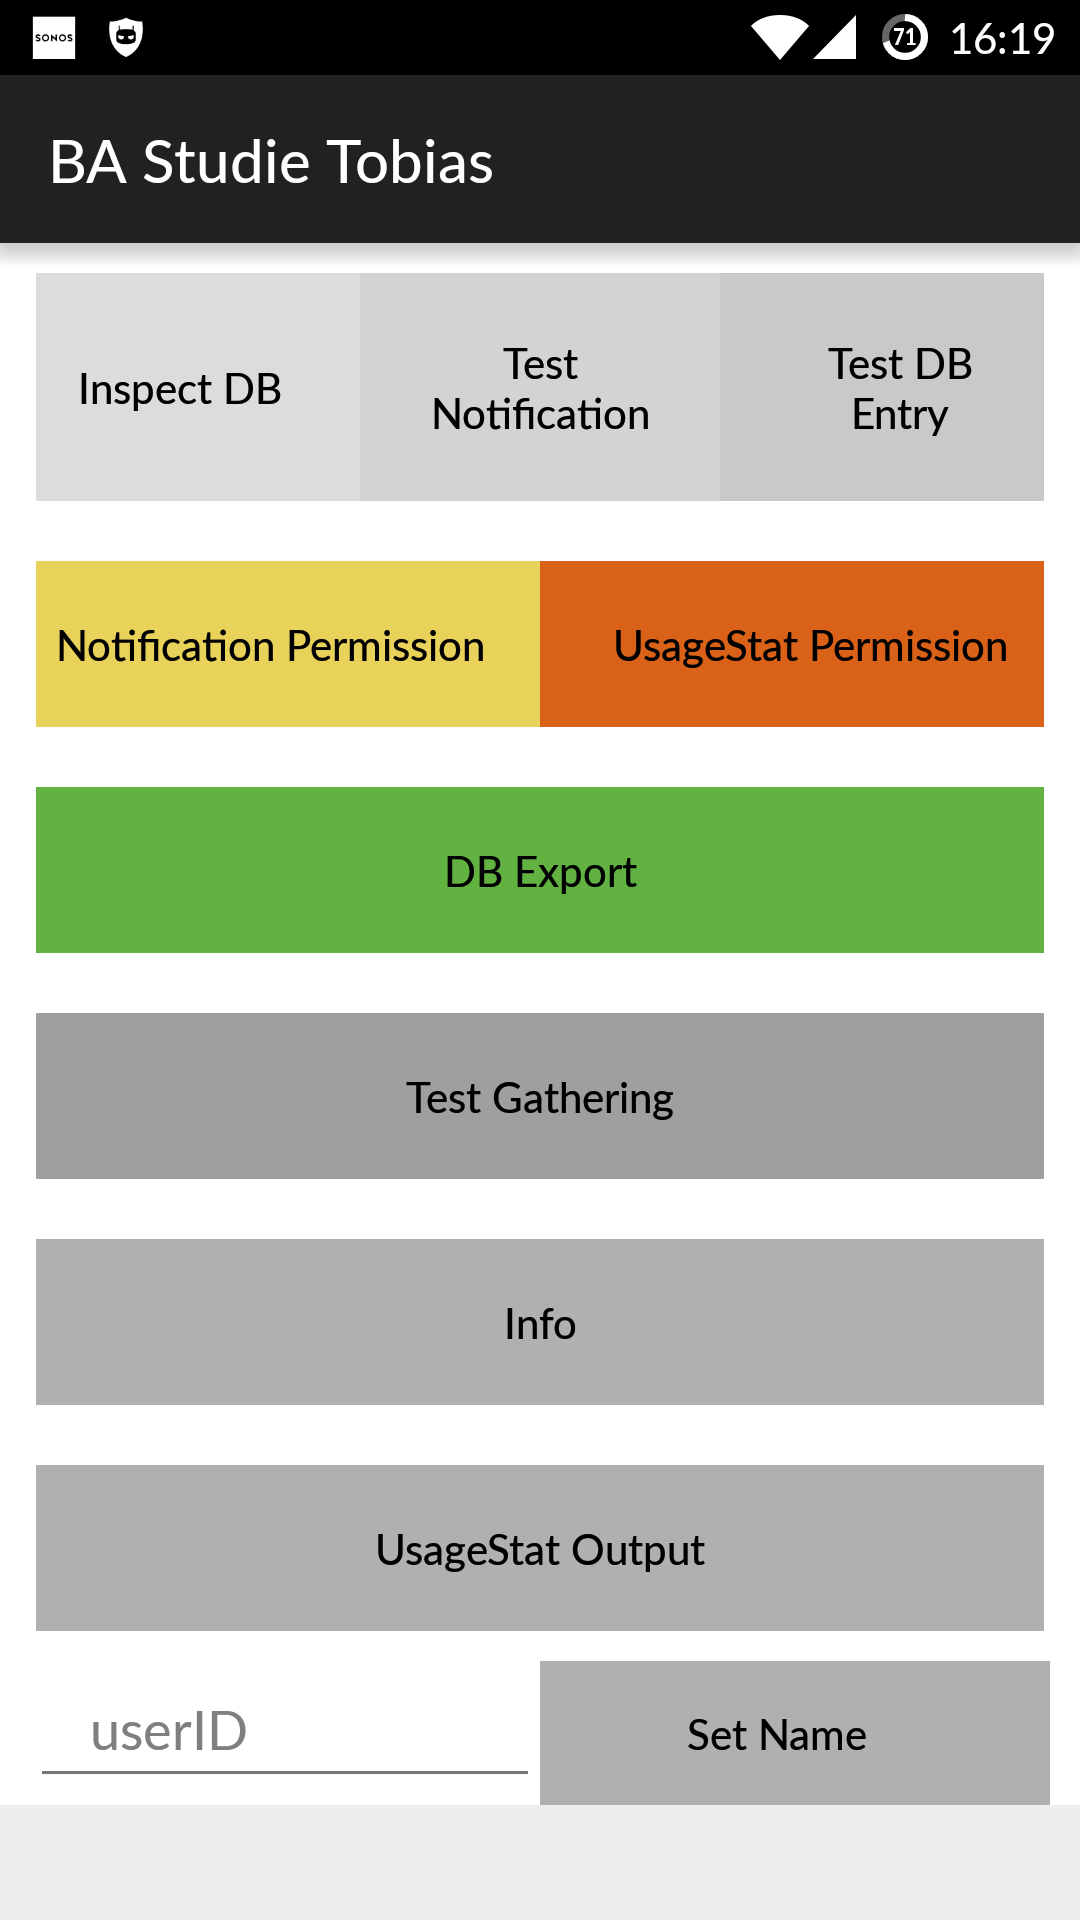
\includegraphics[width=0.7\textwidth]{images/screenshot1.png}
    \caption{User Interface der Applikation}
    \label{fig:uiscreen}
\end{figure}

\section{Call und Message Logs}

Um mit der eigenen Applikation auf die vom Android Betriebssystem gesammelten Logs zu Anrufen und SMS zugreifen zu dürfen, müssen die Berechtigungen 
\textbf{android.permission.READ\_CALL\_LOG} und \textbf{android.permission.READ\_SMS} erteilt werden.
Diese können vom Programmierer in der AndroidManifest.xml Datei beantragt werden und können, da sie keine besonderen Permissions sind,
von der Nutzerin beim Installationsvorgang bestätigt werden.
\par
Mit dem Android \emph{contentResolver} kann nun eine Query durchgeführt werden, mit der die Applikation random read access auf die zurückgegebenen Daten erhält (siehe Code \ref{calllogquery}).
Über diese Daten kann nun iteriert werden und so die gewünschten Features extrahiert werden.
Mit jedem weiteren Eintrag wird die gesamte Anzahl und Gesamtdauer inkrementiert und die spezialisierten Aspekte von INCOMING, OUTGOING und MISSED werden per \emph{switch case} im Falle, dass das aktuelle Item ein ausgehender, ankommender oder verpasster Anruf ist, ebenfalls angepasst.
Die Zählung von einzigartigen Anrufpartnern geschieht hier über eine \emph{HashMap}, die AnruferID auf einen Integerwert mappt, der bei jedem Auftauchen der AnruferID um eins erhöht wird.
Nachdem so über alle Einträge iteriert wurde, werden die gesammelten Daten in einem \emph{CallData} Objekt gespeichert.
\par

Die Message Logs verhalten sich bis auf kleine Details identisch zu den Call Logs und können auf die selbe Weise ausgewertet werden.
Ein Beispiel für ein solches Detail ist unter anderem, das so etwas wie eine verpasste SMS nicht existiert und es nur SENT oder RECIEVED als Möglichkeiten gibt.
Die so gewonnen Daten werden im selben Objekt wie die Daten des Call Logs und werden gemeinsam mit ihnen ausgegeben.

\begin{lstlisting}[frame=single, caption = Call Log Query, label=calllogquery] 
  getContentResolver().query(CallLog.Calls.CONTENT_URI, new String[] { CallLog.Calls.NUMBER, CallLog.Calls.DATE, CallLog.Calls.DURATION, CallLog.Calls.TYPE }, CallLog.Calls.DATE + ">?", new String[] { String.valueOf(resetDate.getTime())}, null);
\end{lstlisting}

\section{NotificationListenerService}

In der \emph{onCreate()} Methode der MainActivity wird der Service, wie in Code \ref{oncreateService} dargestellt, gestartet.
Entsprechend dem Wesen eines Service bei Android läuft dieser nun im Hintergrund weiter, selbst wenn die Applikation, die ihn gestartet hat, stirbt.
Sobald die Nutzerin die entsprechende Berechtigung erteilt, wird bei jeder eingehenden Notification die \emph{onNotificationPosted(StatusBarNotification sbn)} Methode mit der entsprechenden Notification als Argument aufgerufen.
Der NotificationService, der gestartet wurde, ist eine Subklasse des NotificationListenerService, in dem die  \emph{onNotificationPosted()} Methode so überladen wurde,
dass sie zusätzlich so ihrer normalen Funktion noch überprüft ob die absendende Applikation eine der zu betrachtenden Applikationen ist und falls dem der Fall ist, wie in Sektion \ref{ch:Implementierung:sec:Datenbank} beschrieben, einen neuen Eintrag in der Datenbank anlegt.
Dies geschieht wie in Code \ref{validpackage} veranschaulicht durch einen Zugriff auf das im Resourcen System abgelegte Array, das die relevanten Applikationen enthält. 
Das Android Resource System verwaltet alle Nicht-Code Assets der Applikation.
Das so erhaltene Array wird in ein HashSet übertragen, sodass mit dem Aufruf der \emph{contains()} Methode effizient überprüft werden kann ob sich die absendende Applikation unter den relevanten befindet.


\begin{lstlisting}[frame=single, caption = startService(), label=oncreateService] 
  private Intent intentService;
  //...
  intentService = new Intent(this, NotificationService.class);
  startService(intentService);
\end{lstlisting}

\begin{lstlisting}[frame=single, caption = Package Überprüfung, label=validpackage] 
String[] temp = context.getResources().getStringArray(R.array.package_array);
        validPackages = new HashSet<>(Arrays.asList(temp));
\end{lstlisting}



\section{Datenbank}
\label{ch:Implementierung:sec:Datenbank}


Die Datenbank in der die von der Applikation gelesenen Notifications gespeichert werden ist eine SQLite Datenbank.
Dies ist naheliegend, da Android vollständigen Support für SQLite Datenbanken anbietet und wird standardmässig mit SQLite Version 3.4 ausgeliefert.
Die Erstellung der Datenbank wird von \emph{MySQLiteHelper}, einer Subklasse von SQLiteOpenHelper in der \emph{onCreate()} Methode durchgeführt.
An diesem Ort wird auch das Layout der Datenbank ausgewählt:

\begin{lstlisting}[frame=single, caption = Datenbank Strings, label=databasestrings] 
    private static final String DATABASE_NAME = "notificationEntries.db";
    public static final String TABLE_NOTIFICATIONENTRIES = "notificationEntries"; 
    public static final String COLUMN_ID = "_id";
    public static final String COLUMN_NOTIFICATIONENTRY = "notificationEntry";
    public static final String COLUMN_TITLEHASHED = "titelHashed";
    public static final String COLUMN_TEXTLENGTH = "textLength";
    public static final String COLUMN_DATE = "date";
\end{lstlisting}

Hier werden die für das Anlegen der Datenbank relevanten Strings angelegt:
Der Name der Datenbank, der Name der Tabelle in der Datenbank und die Namen der Spalten werden daraufhin daraufhin genutzt, um den SQL Befehl zum Anlegen der Datenbank zusammenzusetzen.

\begin{lstlisting}[frame=single, caption = Datenbank Creation String, label=databasecreation] 
    private static final String DATABASE_CREATE = "create table "
            + TABLE_NOTIFICATIONENTRIES + "(" + COLUMN_ID
            + " integer primary key autoincrement, " + COLUMN_NOTIFICATIONENTRY + " text not null, " + COLUMN_TITLEHASHED + " text not null, " + COLUMN_TEXTLENGTH + " text not null," + COLUMN_DATE + " integer not null);";

\end{lstlisting}

Wie zu sehen, wird hier eine Tabelle namens "`notificationEntries"' angelegt, mit fünf Spalten.
In der ersten Spalte, der Spalte des primären Schlüssels, steht eine eindeutige ID, die mit weiteren hinzugefügten Zeilen selbstständig steigt.
In den restlichen Spalten stehen jeweils die relevanten Inhalte der Notifications also absendende Applikation, der gehashte Titel und die Länge des Notificationtextes, als String und der Timestamp als Integer. 
Hier wird schon bei der Datenbankerstellung festgelegt, dass alle diese Werte nicht leer sein dürfen.

Die überschriebene \emph{onCreate()} Methode führt dann nur noch den hier festgelegten Tabellenerstellungsbefehl auf der Datenbank aus.

\begin{lstlisting}[frame=single, caption = onCreate Methode, label=databaseoncreate] 
  public void onCreate(SQLiteDatabase database) {
        database.execSQL(DATABASE_CREATE);
    } 
\end{lstlisting}

Neue Zeilen in der Tabelle können angelegt werden, indem ein \emph{ContentValues} Object gefüllt 
mit Tupeln aus den Spaltennamen und dem einzutragenden Wert angelegt wird und dieses dann mit der Methode \emph{insert} in die Datenbank eingesetzt wird.

\begin{lstlisting}[frame=single, caption = Einfügen in die Datenbank, label=databaseinsert] 
if (validPackages.contains(pack)) {
            ContentValues values = new ContentValues();
            values.put(MySQLiteHelper.COLUMN_NOTIFICATIONENTRY, pack);
            values.put(MySQLiteHelper.COLUMN_TITLEHASHED, hashedTitle);
            values.put(MySQLiteHelper.COLUMN_TEXTLENGTH, Integer.toString(textSize));
            values.put(MySQLiteHelper.COLUMN_DATE, System.currentTimeMillis());
            database.insert(MySQLiteHelper.TABLE_NOTIFICATIONENTRIES, null,
                    values);
            Log.d("db not", "Updated database");
        }
\end{lstlisting}

Zum Exportieren der Tabelle reicht es eine allgemeine Query auszuführen, die alle Zeilen zurück gibt, wie in Code 
\ref{databaseexport}.

\begin{lstlisting}[frame=single, caption = Einfügen in die Datenbank, label=databaseexport] 
  db.rawQuery("SELECT * FROM " + MySQLiteHelper.TABLE_NOTIFICATIONENTRIES,null); 
\end{lstlisting}

\section{UsageStats}

\section{Export}

Für den Export der gesammelten Daten wird im AndroidManifest.xml die Berechtigung \textbf{android.permission.WRITE\_EXTERNAL\_STORAGE}
benötigt. 
Diese ist keine außergewöhnliche Berechtigung und kann, wie die zum Zugang zu Call und Message Log, bei der Installation der Applikation beantragt werden.
\par
Die gesammelten Daten werden in drei Dateien in einem eigenen Ordner im \emph{ExternalStorageDirectory} des Smartphones gespeichert werden.
Sie werden als Comma Separated Values (csv) gespeichert.
Die Daten werden in die drei Dateien getrennt:

\begin{enumerate}
  \item Die Liste der erhaltenen Notifications
  \item Ergebnisse der Auswertung von Call Log und Message Log
  \item UsageStat Daten
\end{enumerate}
%nach Notification Daten, Anruf beziehungsweise SMS Daten und UsageStat Daten,

Dies geschieht um das potenziell automatisierte Auswerten im Rahmen der Evaluation zu vereinfachen.
\par

Mit Hilfe von OpenCSV, einer einfachen Library zum Lesen und Schreiben von CSV Dateien \cite{opencsv},
wird zunächst die gesamte SQL Tabelle \textbf{TABLE\_NOTIFICATIONENTRIES} wie in Code \ref{databaseexport} angefragt und dann zeilenweise in eine Datei geschrieben.
Der Inhalt des callData Objekts wird als String entgegengenommen und nachdem es in einen StringArray gesplittet wurde, spaltenweise in die zweite Datei geschrieben.
In die dritte Datei werden die UsageStat Daten spaltenweise unter die zugehörigen Package Namen geschrieben.
\par
An alle Dateinamen wird die UserID der Nutzerin, aus der SharedPreference in der sie gespeichert wird, als Suffix angehängt um eine Zuordnung der Daten zu den Auswertungsergebnissen der Fragebögen zu ermöglichen.


\section{Geräte Tests}

Da nicht davon ausgegangen werden kann, dass alle Probandinnen über Smartphones mit vergleichbarer Leistung verfügen, muss die Applikation auch auf weniger leistungsstarken Geräten einwandfrei funktionieren.
Dies ist notwendig, um den komplikationsfreien Ablauf der Studie zu gewährleisten und mögliche Verluste von gesammelten Daten zu vermeiden.
Um dies zu sicher zu stellen wurde die Applikation auf zwei Geräten an verschiedenen Enden des Leistungsspektrums getestet:
Einerseits auf dem OnePlus One Smartphone, als primäres Entwicklungsgerät und Vertreter der leistungsstärkeren Smartphones und andererseits einem Motorola E (2nd Generation) als Vertreter für weniger leistungsstarke Smartphones eingesetzt wurde.
Wichtig waren hierbei die verschiedenen Spezifikationen:
Das OnePlus One ein Smartphone mit einem aktuellen 2.5GHz Quad-Core CPU, 3GB RAM und einem 5,5 Zoll 1920x1080 Pixel Display \cite{oneplusone}
während das Moto E (2nd Gen) als Vertreter der unteren Mittelklasse einen 1.2GHz Quad-Core CPU, 1GB RAM und ein 4,5 Zoll 540x960 Pixel Display hat \cite{motoe}.
Ebenso ist verfügt das OnePlus Ones mit einem Akku mit 3100mAh über mehr Energiereserven als das Moto E, dessen Akku über nur 2390mAh verfügt.
\par
Die Gerätetests waren erfolgreich, das Ausführen der Applikation beanspruchte auch auf dem signifikant schwächeren Gerät keine bemerkbaren Mengen an Ressourcen.



\section{Vorstudie}

Gegen Ende der Implementierung, nach dem groben Testen aller zu implementierenden Funktionalitäten, wurde eine kleine Vorstudie durchgeführt.
Dies geschah um potenzielle Probleme bei der Hauptstudie frühzeitig zu entdecken und zu beheben, bevor sie negativen Einfluss auf die eigentliche Studie nehmen können.
Dazu wurde eine Vorabversion der entwickelten Applikation bei drei freiwilligen Testprobandinnen installiert.
Sie sollten über fünf Tage die Applikation im Hintergrund laufen lassen, sie auf Fehlverhalten untersuchen und die von der Applikation gesammelten Daten validieren.
Alle drei Freiwillige sind Informatikstudentinnen, zwischen 21 und 25 Jahren alt und regelmässige Smartphone User, mit jeweils mehreren aktiv benutzten Kommunikationsapplikationen.
Die verwendeten Smartphones waren jeweils ein OnePlus One, ein OnePlus Two und ein Google Nexus 5.
\par
Jede der drei Freiwilligen bestätigte, dass die von der Applikation aufgezeichneten Daten korrekt waren.
Angemerkt wurde jedoch, dass das Userinterface relativ unübersichtlich sei und selbst mit Instruktionen, wie die Applikation aufzusetzen sei, dies, vorallem für weniger technologieaffine Probandinnen, relativ fehleranfällig sein könnte.
Eine der Probandinnen bemerkte, dass ein nicht zu vernachlässigender Teil ihrer Kommunikation, die über eine Applikation namens Signal laufe, nicht aufgezeichnet werde.
Auch die Wahl der Twitterclients wurde als nicht repräsentativ angemerkt:
Der Twitterclient "`Falcon Pro"' solle berücksichtigt werden.
Positiv wurde bemerkt, dass die Applikation nach dem Aufsetzen sehr ressourcensparend sei und keinerlei zusätzliche Interaktion von der Nutzerin benötigt.
Bei keiner der Freiwilligen kam es zu Abstürzen oder nicht vorgesehenem Verhalten. Auch nach mehrfachem Neustarten verrichtete die Applikation ihre Dienste wie beabsichtigt.
\par
Als Reaktion auf das Feedback aus der Vorstudie wurden folgende Dinge an der Applikation geändert:
Das Interface wurde überarbeitet und in einen übersichtlicheren, harmonischeren Zustand gebracht
In diesem Rahmen wurden für das Aufsetzen relevante Buttons durch farbliches Hervorheben kenntlich gemacht.
Die betrachteten Applikationen wurden um \emph{Falcon Pro}, einen weiteren Drittentwickler Twitterclient, und \emph{Signal}, einen allgemeine Kommunikationsapplikation mit starken Verschlüsselungs und Datenschutzfeatures, erweitert.
%Die Auswahl der zu betrachtenden Applikationen ist bereits so implementiert worden, dass man potenziell später ohne größere Probleme noch etwas hinzufügen oder entfernen kann.
Schon bei dem Entwurf der Applikation wurde darauf geachtet das Hinzufügen und Entfernen von betrachteten Applicationen einfach zu gestalten.
Ansonsten wurde auf die Existenz des Android Features "`Privacy Guard"' hingewiesen, bei dem von der Testprobandin vermutet wurde, es könne mit dem Datensammeln interferieren.
Dies war jedoch nicht der Fall.
\par
Beim Versuch des Übertragens der Daten auf einen Computer kam ein Konflikt mit einem älteren Bug des Android Betriebssystems auf, der von Google im Oktober 2012 anerkannt wurde, jedoch bis heute nicht gefixt wurde
\cite{androidbug}.
Während dieser Bug der eigentlichen App keine Probleme bereitet, erspart Kenntnis dieses Umstandes potenziellen Testprobandinnen eventuelle Unannehmlichkeiten und damit verbundene Frustration beim zurückführen der gesammelten Daten.


%%% Local Variables: 
%%% mode: latex
%%% TeX-master: "diplarb"
%%% End: 
    % Implementierung
%% eval.tex
%% $Id: eval.tex 5 2005-10-10 20:55:48Z bless $

\chapter{Evaluierung}
\label{ch:Evaluierung}
%% ==============================
Hier kommt der Nachweis, dass das in Kapitel~\ref{ch:Entwurf}
entworfene Konzept auch funktioniert. Leistungsmessungen einer
Implementierung werden auch immer gerne gesehen.

Bla fasel\ldots

%% ==============================
\section{Probandinnen}
%% ==============================
\label{ch:Evaluierung:sec:Abschnitt1}

Die Studie wurde begonnen mit 25 Probandinnen.
Alle Probandinnen waren Studentinnen und zwischen 20 und 26 Jahren alt.
Davon studieren 20 Probandinnen Informatik. 
Von den 25 Probandinnen waren 6 weiblich und 19 männlich.
Die Smartphones von drei Probandinnen verfügten über Android Marshmallow, während die 22 verbleibenden Probandinnen über Android Lollipop verfügten.  
Aufgrund von äußeren Umständen sind zwei Probandinnen von der Studie zurücktreten:
Bei einer Probandin gab es einen, von der Studie unabhängigen, kritischen Systemfehler auf ihrem Smartphone, was dazu führte, dass dieses unbenutzbar wurde sie die Studie nicht fortgeführen konnte.
%und sie auf ihr Ersatzsmartphone wechseln musste.
%Dieses ist ein Windows Phone und dementsprechend konnte die Studie dort nicht fortgeführt werden.
Die andere bemerkte zu spät, dass sie nur in einem zu kleinen Zeitfenster and der Studie teilnehmen könnte und trat nach dem Ausfüllen des NEO-PI-R Fragebogens zurück.


%% ==============================
\section{Ablauf}
%% ==============================
\label{ch:Entwurf:sec:Abschnitt2}

Nachdem die Vorstudie, wie im vorangegangenen Kapitel beschrieben, abgeschlossen ist, und potenzielle kleine Änderungen an der Applikation durchgeführt wurden, beginnt die Hauptstudie.
In dieser werden zunächst die Testprobanden ans Teco eingeladen, um dort den NEO-PI-R Fragebogen auszufüllen.
Dazu werden circa drei bis vier Termine innerhalb einer Kalenderwoche angeboten, aus denen die Testprobanden wählen können.
Dies geschieht aus mehreren Gründen. 
Erstens verringert dies, das Risiko, das manche Studienteilnehmerinnen aufgrund von terminlichen Konflikten nicht teilnehmen können.
Zweitens sollen die Daten über einen möglichst ähnlichen Zeitraum gesammelt werden.
Zuletzt ist es so, dass durch das Aufteilen der Probandengruppe eine persönlichere Atmosphäre beim Auftakt der Studie möglich ist
und potenzielle Fragen im Zwiegespräch besser geklärt werden können.
\par
Zu Beginn der Einführung wird den Probandinnen zunächst das Wesen, Bedeutung und potenzielle Tragweite der Studie erläutert.
Potenzielle Risiken und Nutzen werden aufgeführt.
Hier gibt es die Möglichkeit Fragen an die Studienleiterin zu stellen.
Nachdem dies geschehen ist, werden die Probandinnen gebeten, sofern sie nach den Erläuterungen keine Fragen mehr haben und mit der Teilnahme einverstanden sind, eine Einverständniserklärung zu unterschreiben.
Ein zweites Exemplar ist für die Probandin selbst, als von der Studienleiterin unterschriebenen Zusicherung, dass der Rücktritt von den Studie ohne Angabe von Gründen und ohne Nachteile für die Probandin zu jedem Zeitpunkt möglich ist.
Sobald dies abgehandelt ist, können die Probandinnen beginnen den NEO-PI-R Persönlichkeitstest auszufüllen.
Bevor dies geschieht, sollen die Probanden ein selbstgewähltes Pseudonym auf die zweite Seite des Tests schreiben, sodass die gesammelten Daten zu den Tests zugeordnet werden kann, ohne die Anonymität der Probandinnen einzuschränken.
Das alles wird je nach Bearbeitungsgeschwindigkeit ungefähr 35 bis 45 Minuten einnehmen.
\par
Nachdem diese verstrichen sind, und alle Probandinnen ihren Test abgeschlossen haben, werden auch diese eingesammelt.
Nun kann die Applikation auf den mitgebrachten Smartphones der Probandinnen installiert werden.
Im Vorhinein ist die APK der Applikation so in der Cloud hinterlegt worden, dass sie per Scannen eines QR Codes (siehe Abbildung \ref{fig:qrcode}) heruntergeladen werden kann.
Die Installation der Applikation von der APK läuft ab, wie jede andere Applikationsinstallation auf einem Android Gerät auch.
Potenziell muss hier jedoch kurzzeitig die Installation von Applikationen aus nicht verifizierten Quellen freigeschaltet werden, sollte dies nicht sowieso schon der Fall sein.
Nach dem Bestätigen der Basis Berechtigungen ist die Applikation installiert.
Um sie betriebsbereit zu machen müssen die Nutzerinnen die erweiterten Berechtigungen von Hand erteilen.
Dadurch sollte die Applikation betriebsbereit sein.
\par
Um die ordnungsgemäße Funktionstüchtigkeit zu gewährleisten sind in der Applikation Tests implementiert, die nun durchgeführt werden sollen.
Sind diese erfolgreich durchgeführt worden, so beginnt der Datensammelungszeitraum der Studie.
Dieser endet zwischen 10 und 20 Tagen später.
Nachdem die von der Applikation gesammelten Daten exportiert und zurück bei der Studienleiterin angekommen sind, 
ist die Studie beendet.

\begin{figure}[h]
    \centering
    
\includegraphics{images/qrcode.png}
    \caption{QR Code}
    \label{fig:qrcode}
\end{figure}


%% ==============================
\section{Probleme während dem Studienablauf}
%% ==============================

Gleich zu Beginn der Studie, bei der Installation der Applikation gab es bei einer Probandin Probleme mit der Android Version:
Der Optionspunkt in der einer Applikation der Zugang zu den UsageStat Daten ermöglicht, wurde vom Hersteller auf dem LG Gerät zumindest in der Default ROM ersatzlos entfernt.
Dies führt dazu, dass die Datensammelapplikation der Studie nicht auf alle Daten Zugriff bekommt, auf die sie Zugriff benötigt.
Die Probandin, selbst eine Android Programmiererin, die mehrere aktuelle Android Smartphones besitzt, bot daraufhin an für die Dauer der Studie auf ein anderes Gerät umzusteigen.
Ein einfaches Überführen der SIM Karte in das Zeitgerät umgeht das Problem.
\par
Im Verlauf der Studie beobachteten mehrere Probandinnen,  dass die von der App erhaltenen Werte für die Vordergrundzeit verschiedener Applikationen ungenau oder zu gering seien.
Dies scheint unabhängig von der sammelnden Applikation zu sein, sondern ein unerwartetes Verhalten des Android Betriebssystems selbst, dass falsche Daten aus der Schnittstelle ausgibt.
Aufgrund der Unzugänglichkeit der Problematik und Zeitbedenken wurden, nach Rücksprache mit der betreuenden Mitarbeiterin, die gesammelten UsageStat Daten für unzuverlässig erklärt.
Dementsprechend werden diese Daten in der Evaluation nicht mehr berücksichtigt.
\par
Nach Ablauf der geplanten Studienzeit bekamen alle Studienteilnehmer die Aufforderung die gesammelten Daten zu exportieren und der Studienleiterin zukommen zu lassen. 
In 20 von 23 Fällen funktionierte dies perfekt.
Jedoch gab es einen Fall, in dem das bereits aufgefallene Problem \cite{androidbug} mit der Android Dateiübertragung auftrat.
Dies konnte die Probandin nach einem Hinweis durch einen Neustart des Geräts beheben.
Die anderen beiden Fälle wurden durch zerstreute Probandinnen und das System der Anonymisierung beziehungsweise Pseudonymisierung hervorgerufen.
Da der Studienleiterin nur die Pseudonyme der Probandinnen bekannt waren, gestaltete es sich unmöglich die beiden fehlenden Probandinnen direkt auf das Fehlen ihrer Datensätze hinzuweisen.
Mit sieben Tagen Verspätung und nach etlichen Nachrichten an verschiedene Teilnehmerinnen waren die gesammelten Daten dann vollständig.

\section{Feedback}

Nach Abschluss der Studie wurden die Probandinnen dazu aufgefordert einen kurzen Feedback Fragebogen auszufüllen.
Die gestellten Fragen "`Hat sich die Nutzung Ihres Smartphones während der Studie/durch die App verändert? Wie?"', "`Welche Kommunikations- oder Social Media-Apps verwendest du noch, welche nicht mitgeloggt wurden?"' und "`Freies Feedback: Gibt es noch etwas, dass ihr mir sagen möchtet?"' waren alle drei als Freitext Fragen gestellt.
\par
Die Antworten bezüglich der ersten Frage waren ausnahmslos verneinend.
Der Grund hierfür ist vermutlich bei der Abwesenheit von Interaktion mit der Applikation zu finden.
Die Abwesenheit von Interaktion wurde sogar beim freien Feedback einmal explizit als positiv hervorgehoben und die Applikation wurde als "`nicht bemerkbar"' beschrieben.
\par
Antworten auf die zweite Frage waren dann schon weniger homogen:
Mehrere Probandinnen wiesen hier auf "`Conversations"' hin. 
Das ist ein Android Jabber / XMPP Client, mit dem verschiedene Dienste, die das XMPP Übertragungsformat nutzen, in einer App bündeln kann.
Viele Einstellungsmöglichkeiten, wie zum Beispiel die Verschlüsselung über OTR oder OpenPGP, machen diese Applikation für den Normalnutzer eher unhandlich, für Informatikstudentinnen aber umso attraktiver.
Angesichts der am Ende doch sehr Informatik lastigen Probandinnen wäre die Aufnahme dieser App in die Liste der zu betrachtenden Apps durchaus zu rechtfertigen gewesen.
Einige obskure Twitterclients wurden noch angeführt.
Aufgrund der schieren Masse an verschiedenen Twitter Applikationen ist es schwerlich möglich diese alle von Entwicklerseite abzudecken. 
Im Nachhinein wäre eine denkbare Lösung für dieses Problem, dass der Nutzer selbst eintragen kann, wie das Package des Twitter Clients seiner Wahl heißt.
Da das Ändern von Resource Daten durch Userinput nicht möglich ist, müsste man zwar das Konzept ändern mit dem die relevanten Packagenamen gespeichert werden, doch dies scheint ein lösbares Problem zu sein.
\par
Eine andere Antwort umfasst sowohl die Frage nach nicht mitgeloggten Applikationen, als auch das freie Feedback Feld:
Eine der teilnehmenden Probandinnen ist in Asien geboren und hat noch immer regen kontakt mit Freunden beziehungsweise Familie von dort, 
die selbstverständlich nicht die in Deutschland, beziehungsweise der westlichen Welt herkömmlich benutzten Applikationen benutzen, sondern die Asiatischen.
Beispiele die angeführt wurden waren QQ, WeChat oder Ren Ren.
Demensprechend bemerkte sie, dass insgesamt die Auswahl der betrachteten Applikationen sehr "`westlich"' war.
Während dies unzweifelhalt wahr ist, so ist der Anspruch über Deutschland hinaus solche Muster zu untersuchen sicher etwas außerhalb des Rahmens einer Bachelorarbeit.
Für weitergehende Forschungen ist jedoch sicher viel Platz auf diesem Gebiet, unter anderem vielleicht dem Unterschied zwischen Applikationsverhalten in Europa, Nord- beziehungsweise Süd-Amerika und Asien. 
\par

TODO: Freies Feedback, e.g. DER FRAGEBOGEN

\section{Auswertung der Daten}

Das Umsetzen der erhaltenen Daten in eine aussagekräftige Übersicht war für die gesammelten Call und Message Log Daten nicht notwendig, da sie bereits in einem solchen exportiert werden, für die Liste an Notifications ist dies jedoch dringend notwendig.
Dafür wurde eine Java Command Line Applikation geschrieben, die Daten aus verschiedenen Dateien einließt und am Ende die aggregierten Daten in eine Datei schreibt.
\par
Es wird ein Pfad zu dem Ordner in dem sich die zu betrachtenden Dateien befinden angegeben.
Über alle in sich diesem Ordner befindlichen Datein wird iteriert und für jede wird zunächst der gesamte Inhalt der Datei mit der Methode \emph{readStringFromFile()} in einen String geschrieben.
Mit der \emph{split()} Methode und dem regulären Ausdruck  $(\backslash r?\backslash n)|,|(\backslash t)$ wird der String in die Comma Separated Values aufgeteilt.
Da die ursprüngliche Tabelle 5 Spalten hatte sind nun die Attribute der i. Notification im Array in den Positionen $ [i * 5 + 0]$ bis $ [i * 5 + 4]$ gespeichert.
Diese werden nun in Objekte \emph{Notification} mit den entsprechenden Attributen und einem Enum für die absendende Applikation geparst.
Alle so erstellten Objekte werden dann in eine ArrayList geschrieben auf der weitergearbeitet wird.
Zur einfacheren Werteberechnung für einzelne Applikationen wird nun für jede mögliche Applikation eine eigene ArrayListe angelegt, in die nur die Notifications hinzugefügt werden die die entsprechende Applikation als Absender haben.
Für jede dieser ArrayListen werden nun folgende Werte berechnet:

\begin{itemize}
  \item Anzahl Notifications (Länge der ArrayList)
  \item Anzahl Konversationen (Anzahl einzigartiger Titelhashes)
  \item Größte Konversation (Maximum TextLength)
  \item Durchschnittliche Konversationsgröße (Summe TextLength durch Anzahl Konversationen)
  \item Durchschnittliche Nachrichtenlänge (Summe TextLength durch Anzahl Notifications)
\end{itemize}

Diese Berechnungen werden jeweils in einer Methode, ähnlich zum Beispiel \ref{maxconv} durchgeführt, die dann auf auf alle ArrayLists aufgerufen wird.


\begin{lstlisting}[frame=single, caption =  calculateMaxConversationSize(), label=maxconv] 
    public static int calculateMaxConversationSize(ArrayList<Notification> list) {
        HashMap<String, Integer> hmap = new HashMap<>();
        for (Notification noti : list) {
            if (!hmap.containsKey(noti.getTitle())) {
                hmap.put(noti.getTitle(), 1);
            }
            else {
                hmap.put(noti.getTitle(), hmap.get(noti.getTitle())+ 1);
            }
        }
        if (hmap.size() == 0){
            return 0;
        }
        else {
            return (Collections.max(hmap.values()));
        }

    }
\end{lstlisting}


Über alle Daten werden zusätzlich noch folgende Werte berechnet:

\begin{itemize}
  \item Anzahl Applikationen genutzt (Anzahl ArrayLists mit Size > 0)
  \item Anzahl Notifications insgesamt
  \item Anzahl Notifications pro Tag
  \item Durchschnittliche Nachrichtenlänge gesamt
  \item Meist genutzte Applikation
  \item Applikation mit den meisten Konversationen
  \item Applikation mit den durschnittlich längsten Nachrichten  
\end{itemize}

Die so aggregierten Daten werden dann in eine Datei geschrieben von der sie dann an relevante Stellen übertragen werden können.

\section{Ergebnisse}

Die Auswertung der NEO-PI-R Fragebögen ergab, dass von den 23 Probanden, die letztendlich betrachtet wurden, elf eine durchschnittliche, acht eine sehr niedrige, drei eine hohe und nur einer eine niedrige Geselligkeit hatten.
Auf der Skala von 0 bis 4 lag der Durchschnitt bei ungefähr $1.6$ mit einer Standardabweichung von $0.9$ und zwischen dem Minimum von $0.125$ und dem Maximum von $2.75$.
Im Vergleich dazu Werte der Extraversion:
Im Durchschnitt $1.88$ mit Standardabweichung von $0.57$, dem Minimum bei $0.56$ und dem Maximum bei $2.6$.
Die Verteilung der Ergebnisse ist in Diagramm \ref{fig:neoergebnisse} veranschaulicht.

\begin{figure}[h]
    \centering
    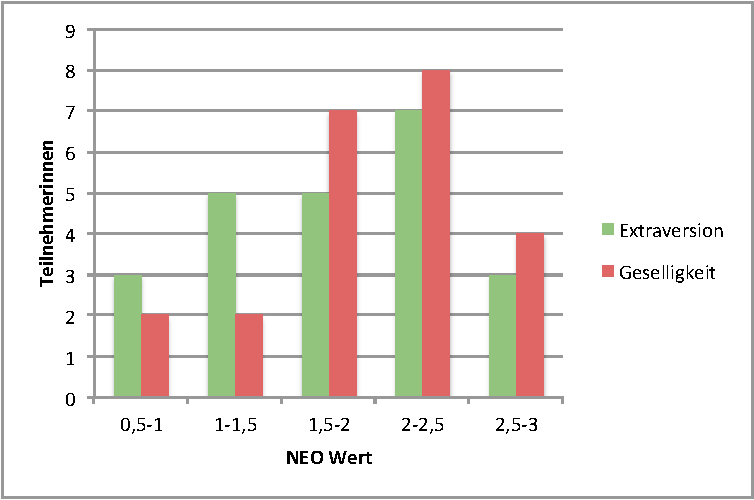
\includegraphics{images/NeoErgebnisse.pdf}
    \caption{Verteilung der Geselligkeit und Extraversion der Probandinnen}
    \label{fig:neoergebnisse}
\end{figure}

Durchschnittlich führten die Probandinnen $0.66$ Telefongespräche pro Tag bei einer Standartabweichung von $0.89$.
Drei Probandinnen führten überhaupt keine Telefongespräche und die Probandin mit der höchsten Telefonnutzung tätigte $4.03$ Anrufe pro Tag.
Das ist eine höhere Nutzung als die von SMS, was im Durchschnitt nur $0.38$ Nachrichten pro Tag bei einer Standardabweichung von $0.6$ war.
SMS wurde von vier Probandinnen überhaupt nicht genutzt und das Maximum lag bei $1.86$ Nachrichten pro Tag.
Die Verteilung von Anrufen und Nachrichten ist in Diagramm \ref{fig:callmessagesdistr} dargestellt.

\begin{figure}[h]
    \centering
    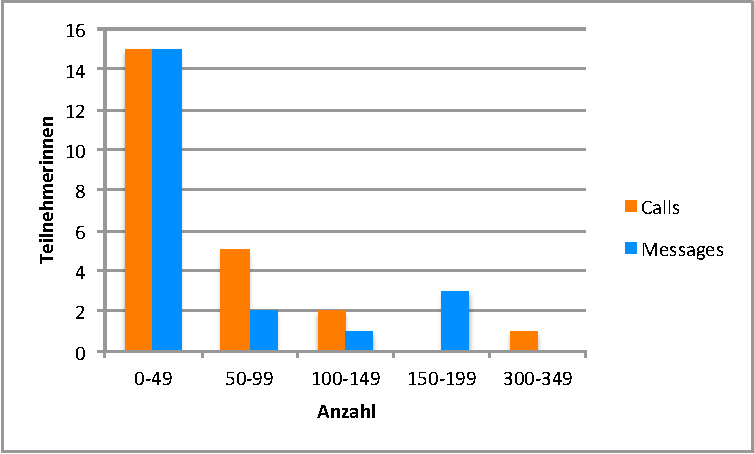
\includegraphics{images/callsMessagesDistr.pdf}
    \caption{Verteilung der Anrufe und Nachrichten der Probandinnen}
    \label{fig:callmessagesdistr}
\end{figure}


Bei den gesammelten Notifications wurden durchschnittlich $157.29$ Notifications pro Tag bei einer Standardabweichung von $378.60$ empfangen.
Dies ist einem extremen Ausreißer geschuldet, der über 17 Tage 31716 Notifications erhalten hat. 
Das sind fast $8.5$ mal mehr als der zweithöchste Wert, mit 3755 Notifications.
Entfernt man diesen Wert aus dem Datenpool reduziert sich der Durchschnitt auf $79.63$ Notifications pro Tag mit einer Standartabweichung von $69.79$
\par
Die Verteilung der meistgenutzten Applikationen jeder Teilnehmerin sind in Diagramm \ref{fig:mostusedapp} dargestellt.
\par
TODO: Beschreibung korrelationen

\begin{figure}[h]
    \centering
    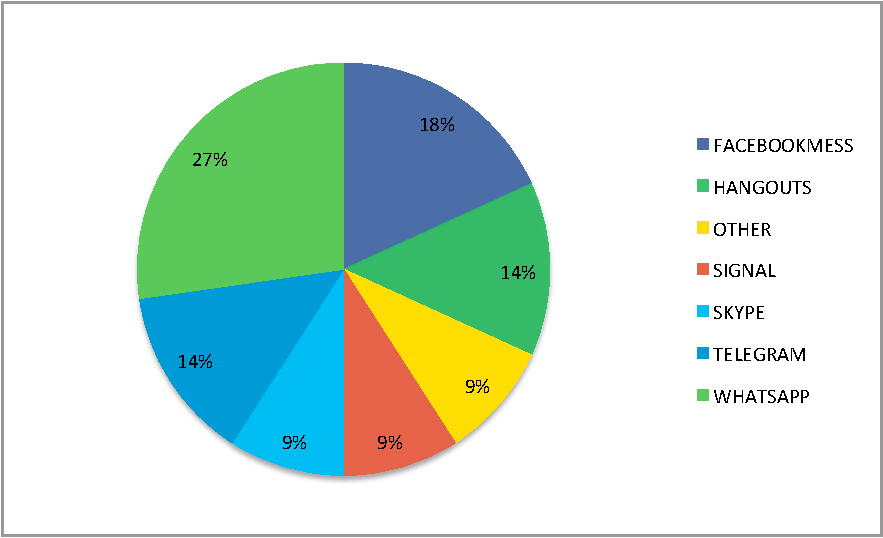
\includegraphics{images/MostUsedApp.pdf}
    \caption{Verteilung der meistgenutzten Applikationen}
    \label{fig:mostusedapp}
\end{figure}



%% ==============================
\section{Zusammenfassung}
%% ==============================
\label{ch:Evaluierung:sec:zusammenfassung}

Am Ende sollten ggf. die wichtigsten Ergebnisse nochmal in \emph{einem}
kurzen Absatz zusammengefasst werden.

%%% Local Variables: 
%%% mode: latex
%%% TeX-master: "diplarb"
%%% End: 
        % Evaluierung
%% zusammenf.tex
%% $Id: zusammenf.tex 4 2005-10-10 20:51:21Z bless $
%%

\chapter{Zusammenfassung und Ausblick}
\label{ch:Zusammenfassung}
%% ==============================


In dieser Arbeit wurde der Zusammenhang zwischen der Geselligkeits- beziehungsweise Extraversions-Facette
einer Persönlichkeit und der Smartphone Nutzung im Kontext von Social Media und Kommunikation untersucht.
Es wurden verwandte Arbeiten vorgestellt und bewertet.
\par
TODO: FUELLEN MIT RELATED WORK
\par
Daraufhin wurde eine Studie entworfen und nach der Durchführung einer kleineren formativen Studie durchgeführt, die anhand 25 Testprobandinnen Daten, aus einem durchgeführten Selbstbeurteilungsfragebogen und
 mittels einer dazu entwickelten Android Applikation, bezüglich dieses Zusammenhangs sammelt.

Folgend darauf wurde das Durchführen der Studie sowie die aufgekommenen Problemen beschrieben und durchgeführte Lösungsansätze diskutiert.
\par
TODO: BESCHREIBUNG STUDIE
\par
Die so gesammelten Daten konnten belegen, dass *INSERT THESE HIER*.\\
*so viele Datendinge hier*\\
*ganz viele*
\par
TODO: AUSBLICK AUF DIE ZUKUNFT!
\par
Abschließend kann man sagen, dass die große Menge an personenbezogenen Daten,
die jeden Tag durch das persönliche Smartphone fließt, dieses zu einem sehr attraktiven Werkzeug zur Betrachtung der Persönlichkeit seiner Benutzerin macht.
Dies begrenzt sich nicht nur auf die Geselligkeit oder die Extraversion: Die Aspekte die nicht so betrachtet werden können sind verschwindend wenige.
Dies ist ein interessantes Forschungsthema, mit viel Potenzial in der Zukunft, jedoch muss Acht gegeben werden.
Diese Forschung kann leicht den Vorteil der Nutzerin aus den Augen verlieren und missbraucht werden. 


%%% Local Variables: 
%%% mode: latex
%%% TeX-master: "diplarb"
%%% End: 
   % Zusammenfassung und Ausblick

%% ++++++++++++++++++++++++++++++++++++++++++
%% Anhang
%% ++++++++++++++++++++++++++++++++++++++++++

\appendix
%\include{anhang_a}
%\include{anhang_b}

%% ++++++++++++++++++++++++++++++++++++++++++
%% Literatur
%% ++++++++++++++++++++++++++++++++++++++++++
%  mit dem Befehl \nocite werden auch nicht 
%  zitierte Referenzen abgedruckt
\cleardoublepage
\phantomsection
\addcontentsline{toc}{chapter}{\bibname}
%%
\nocite{*} % nur angeben, wenn auch nicht im Text zitierte Quellen 
           % erscheinen sollen
\bibliographystyle{itmabbrv} % mit abgekürzten Vornamen der Autoren
%\bibliographystyle{gerplain} % abbrvnat unsrtnat
% spezielle Zitierstile: Labels mit vier Buchstaben und Jahreszahl
%\bibliographystyle{itmalpha}  % ausgeschriebene Vornamen der Autoren
\bibliography{diplarb}
%% ++++++++++++++++++++++++++++++++++++++++++
%% Index
%% ++++++++++++++++++++++++++++++++++++++++++
\ifnotdraft{
\cleardoublepage
\phantomsection
\printindex            % Index, Stichwortverzeichnis
}
\end{document}
%% end of file
